\documentclass[11pt]{article}

\usepackage{amssymb,amsmath,amsfonts,amsthm}
\usepackage{lmodern}
\usepackage{xcolor}
\usepackage[colorlinks=true]{hyperref}
\definecolor{cieblue}{RGB}{31, 119, 180}
\hypersetup{
    citecolor=cieblue,
    allcolors=cieblue
}
\usepackage{mathtools}
\usepackage{enumerate}
\usepackage{booktabs}
\usepackage{float}
\usepackage[ruled]{algorithm2e}
\usepackage{tikz}

\setlength{\textwidth}{15.5cm} \setlength{\headheight}{0.5cm} \setlength{\textheight}{21.5cm}
\setlength{\oddsidemargin}{0.25cm} \setlength{\evensidemargin}{0.25cm} \setlength{\topskip}{0.5cm}
\setlength{\footskip}{1.5cm} \setlength{\headsep}{0cm} \setlength{\topmargin}{0.5cm}

\newtheorem{definition}{Definition}[section]
\newtheorem{proposition}{Proposition}[section]
\newtheorem{lemma}{Lemma}[section]
\newtheorem{theorem}{Theorem}[section]
\newtheorem{corollary}{Corollary}[section]
\newtheorem{remark}{Remark}[section]
\newtheorem{example}{Example}[section]

\newcommand{\Z}{\mathbb{Z}}
\newcommand{\R}{\mathbb{R}}
\newcommand{\N}{\mathbb{N}}
\newcommand{\Pic}{\operatorname{Pic}^0}
\newcommand{\Div}{\operatorname{Div}^0}
\newcommand{\im}{\operatorname{im}}
\newcommand{\tw}{t_{\mathrm{w}}}
\newcommand{\pbar}{\bar{p}}
\newcommand{\norm}[1]{\left\lVert#1\right\rVert}

\allowdisplaybreaks

\begin{document}

\title{Improving the Marked Edge Walk via\\Fiber Decomposition and Gradient-Biased Proposals}
\author{Alaittin K\i rt\i \c{s}o\u{g}lu}
\footnotetext[1]{Department of Applied Mathematics, Illinois Institute of Technology}
\maketitle

\tableofcontents


%═══════════════════════════════════════════════════════════════════════════════
\section{Problems with MEW}\label{sec:problems}
%═══════════════════════════════════════════════════════════════════════════════

We identify two structural inefficiencies in the Marked Edge Walk (MEW)
that worsen with problem size.

\medskip\noindent
\textbf{(P1) Within-fiber waste.}
MEW's cycle basis step picks a non-tree edge $e^+$ uniformly from \emph{all}
non-tree edges. On an $N \times N$ grid with $d = 4$ quadrant districts,
the fraction of non-tree edges that are interior (both endpoints in the same
district) is $f_{\mathrm{int}} = 1 - 1/(N-1)$, which exceeds $80\%$ on a
$6 \times 6$ grid and $96\%$ on $30 \times 30$. Swapping along the fundamental
cycle of an interior edge cannot change the partition. We call these
\emph{within-fiber} steps: they shuffle the spanning tree within the same
equivalence class of compatible trees (Section~\ref{sec:fiber}) without
producing any partition exploration.

For each grid size $N \in \{6, 10, 15, 20, 25, 30\}$, we build the
$N \times N$ grid graph, partition into $d = 4$ quadrants, sample an initial
spanning tree via Wilson's algorithm, and run $10{,}000$ MEW cycle basis steps.
After each step, we record whether the boundary signature (the set of tree
edges crossing district boundaries) changed.

\begin{table}[H]
\centering
\begin{tabular}{crrrrrr}
\toprule
Grid & $n$ & Waste & Speedup & $\log t(G)$ & $\log \prod_i t(G[\xi_i])$ & $\log$ ratio \\
\midrule
$6 \times 6$   &   36 & --\% &  --$\times$ &  -- & -- & -- \\
$10 \times 10$ &  100 & --\% &  --$\times$ &  -- & -- & -- \\
$15 \times 15$ &  225 & --\% &  --$\times$ &  -- & -- & -- \\
$20 \times 20$ &  400 & --\% &  --$\times$ &  -- & -- & -- \\
$25 \times 25$ &  625 & --\% &  --$\times$ &  -- & -- & -- \\
$30 \times 30$ &  900 & --\% &  --$\times$ &  -- & -- & -- \\
\bottomrule
\end{tabular}
\caption{Waste fraction and spanning tree scaling with grid size ($d = 4$ quadrant
districts). Waste is the fraction of MEW cycle basis steps that do not change the
boundary signature; Speedup $= 1/(1-\text{Waste})$. The log ratio
$\log t(G) - \log \prod_i t(G[\xi_i])$ measures the cross-boundary state space
size.}\label{tab:scaling}
\end{table}

\begin{proposition}[Waste fraction scaling]\label{prop:waste-scaling}
For the $N \times N$ grid with $d = 4$ quadrant districts, the waste fraction
$\rho(N)$ satisfies
\[
  \rho(N) \;\to\; 1 \quad \text{as } N \to \infty,
\]
and the empirical data is well-approximated by $\rho(N) \approx f_{\mathrm{int}}(N) = 1 - 1/(N-1)$.
\end{proposition}

\begin{proof}[Heuristic argument]
A cycle basis step picks a uniformly random non-tree edge $e^+$. The probability
that $e^+$ is a boundary edge is at most $|\partial\xi|/|E \setminus T|$, where
$|E \setminus T| = m - (n-1) = g$ is the number of non-tree edges (the genus).
Even if $e^+$ is a boundary edge, the fundamental cycle may swap it for another
boundary edge, leaving the boundary signature unchanged. Conversely, if $e^+$ is
an interior edge, the step can only change the boundary signature if the
fundamental cycle passes through boundary edges and the randomly selected
$e^-$ happens to be one of them.

As $N$ grows, $|\partial\xi| = 2N$ while $g = m - n + 1 = 2N(N-1) - N^2 + 1
= N^2 - 2N + 1 = (N-1)^2$. The fraction of non-tree edges that are boundary
edges is at most $2N/(N-1)^2 \to 0$, so the probability that any given step
touches the boundary vanishes. This explains why the waste fraction approaches
$1$.
\end{proof}

\medskip\noindent
\textbf{(P2) Blind marked-edge selection.}
To understand the relative contribution of the cycle step and the marked edge
step to partition exploration, we classify every MEW step on the $6 \times 6$
grid into four cases based on whether the quotient tree (the set of
boundary tree edges) and the partition change. The quotient tree
captures the cross-boundary structure; two spanning trees with the same quotient
tree differ only in their within-district edges.

We run $50{,}000$ full MEW steps (cycle basis step $+$ marked edge step) on the
$6 \times 6$ grid with $d = 4$ quadrant districts. After each step, we record
the quotient tree and partition.

\begin{table}[H]
\centering
\begin{tabular}{clccr@{\hspace{8pt}}rr}
\toprule
Case & Description & QT & Partition & Count & \% & New discoveries \\
\midrule
A & Boundary jump              & changed & changed & -- & --\% & -- \\
B & Local adjustment (via $M$) & same    & changed & -- & --\% & -- \\
C & QT change, same partition  & changed & same    & -- & --\% & --- \\
D & No change                  & same    & same    & -- & --\% & --- \\
\bottomrule
\end{tabular}
\caption{Classification of MEW steps on the $6 \times 6$ grid by quotient tree (QT)
and partition change. New discoveries counts steps that reach a partition not
previously visited.}\label{tab:step-class}
\end{table}

\begin{enumerate}
  \item Case C = 0: every quotient tree change produces a partition
    change. Boundary moves are never wasted.

  \item Case D $\approx$ 43\%: nearly half of all MEW steps change neither
    the quotient tree nor the partition. These are the within-fiber moves
    of~(P1).

  \item Case A vs.\ B: among steps that change the partition,
    $\sim 85\%$ come from boundary jumps (the cycle step changes the quotient
    tree) and only $\sim 15\%$ from local adjustment (the marked edge step
    slides $M$ within the same quotient tree). The cycle step is the primary
    driver of partition exploration, yet MEW's random walk on marked edges
    treats all tree edges equally.

  \item Discovery rate: boundary jumps discover $\sim 78\%$ of all new
    partitions, but $\sim 80\%$ of boundary jumps revisit previously seen
    partitions. This high revisit rate reflects
    the locality of MEW's single-edge-swap moves.
\end{enumerate}

\begin{remark}[Comparison with ReCom's exploration pattern]
ReCom's merge-and-resplit step completely resamples a spanning tree of the
merged subgraph, producing a partition that can be very different from the
current one. MEW's cycle step swaps one edge at a time, making incremental
changes to the quotient tree.
The advantage of MEW is not mixing speed but the ability to target arbitrary
distributions via calculable transition probabilities~\cite{mew}.
\end{remark}


%═══════════════════════════════════════════════════════════════════════════════
\section{Our Approach}\label{sec:algorithm}
%═══════════════════════════════════════════════════════════════════════════════

We modify the MEW framework to address both problems:
\begin{itemize}
  \item Step~1 (boundary cycle step) solves \textbf{(P1)} by restricting
    $e^+$ to boundary non-tree edges and biasing selection toward edges with
    high population gradient. Every proposal changes the partition.
  \item Step~2 (QP-guided marked edge selection) solves \textbf{(P2)} by
    replacing MEW's blind random walk on marked edges with a quadratic program
    that directly targets population balance.
\end{itemize}

Fix a connected graph $G = (V, E)$ with populations $\{p_v\}$, number of
districts $d$, ideal population $\pbar = \frac{1}{d}\sum_v p_v$, and balance
tolerance $\varepsilon > 0$.

\begin{definition}[Feasible partition]\label{def:feasible}
A $d$-partition $\xi$ is \emph{feasible} if each district is connected and
population-balanced:
\[
  |p(\xi_i) - \pbar| \leq \varepsilon \, \pbar \quad \text{for all } i,
\]
where $p(\xi_i) = \sum_{v \in \xi_i} p_v$.
\end{definition}

The chain operates on the MEW state space $\mathcal{X} = \{(T, M)\}$ where
$T$ is a spanning tree of $G$ and $M \subset E(T)$ with $|M| = d - 1$ is the
marked edge set. The forest $T \setminus M$ defines a $d$-partition
$\xi(T, M)$.

A non-tree edge $e \in E(G) \setminus E(T)$ is a \emph{boundary non-tree edge}
if its endpoints lie in different districts of $\xi$.

\subsection{The Boundary Cycle Step}

The key observation is that MEW's cycle basis step picks $e^+$ uniformly from
\emph{all} non-tree edges. On an $N \times N$ grid, $65\%$--$94\%$ of non-tree
edges are interior (both endpoints in the same district), and swapping along
their fundamental cycle cannot change the partition. Two fixes are applied:
restrict $e^+$ to boundary non-tree edges, and bias selection
toward edges with high population gradient.

\subsubsection*{Pre-computation: Population Potential}

Define the \emph{district imbalance source} for each node $v \in V$ with
$\xi(v) = i$:
\[
  b_v = \frac{p(\xi_i) - \pbar}{|\xi_i|}.
\]
Nodes in overpopulated districts act as sources; nodes in underpopulated
districts act as sinks. The vector $b$ satisfies $\sum_v b_v = 0$.

Solve the Poisson equation $\Delta_G \phi = b$ for the \emph{population
potential} $\phi \in \R^V$. The gradient $|\phi(u) - \phi(v)|$ across each
edge $(u,v)$ measures the inter-district population pressure: edges with large
gradients are natural partition boundaries separating surplus from deficit
districts. For planar redistricting graphs, the sparse Cholesky factorization
of $\Delta_G$ costs $O(n^{3/2})$ and each back-solve is $O(n)$. The potential
$\phi$ is recomputed when the partition changes.

\begin{algorithm}[H]
\caption{MEW with Boundary Cycle Step}\label{alg:boundary-cycle}
\KwIn{State $(T, M)$ with feasible partition $\xi = T \setminus M$;
population potential $\phi$}
\KwOut{New state $(T', M')$}
\BlankLine
\tcc{Step 1: Gradient-biased boundary cycle step}
$B \gets \{e \in E(G) \setminus E(T) : \xi(e_0) \neq \xi(e_1)\}$\;
Select $e^+ \in B$ with $P(e^+) = \dfrac{|\phi(e^+_0) - \phi(e^+_1)|}
  {\sum_{e \in B} |\phi(e_0) - \phi(e_1)|}$\;
$C \gets$ fundamental cycle of $e^+$ in $T$\;
Select $e^- \in C \setminus (M \cup \{e^+\})$ uniformly at random\;
\lIf{no such $e^-$ exists}{\Return{$(T, M)$}}
$T' \gets (T \cup \{e^+\}) \setminus \{e^-\}$\;
\BlankLine
\tcc{Step 2: QP-guided marked edge selection}
\ForEach{$e \in T'$}{
  Compute subtree population $\sigma_e$ and rebalancing flow
  $f_e = \sum_{u \in \mathrm{subtree}(e)} b_u$\;
}
Solve QP: $\min\; x^\top Q\, x + c^\top x$ s.t.\
$\sum x_e = d-1$, $x \in [0,1]^{n-1}$\;
$M' \gets$ $d-1$ edges with largest $x_e$\;
\lIf{$\xi' = T' \setminus M'$ is not feasible}{\Return{$(T, M)$}}
\BlankLine
\tcc{Step 3: Acceptance}
$\alpha \gets \min\!\Bigl(1,\;
  \frac{P'(e^-)}{P(e^+)} \cdot
  \frac{|C \setminus (M \cup \{e^+\})|}{|C' \setminus (M' \cup \{e^-\})|}\Bigr)$\;
Accept $(T', M')$ with probability $\alpha$; otherwise keep $(T, M)$\;
\end{algorithm}

\medskip\noindent
All three components of the MEW transition are modified. Step~1 restricts
$e^+$ to boundary non-tree edges (eliminating within-fiber waste,
Section~\ref{sec:problems}) and biases selection toward high population-gradient
edges via the Laplacian potential $\phi$. Step~2 replaces MEW's blind random
walk on marked edges with QP-guided selection that directly targets population
balance.
Ergodicity over the full state space $\{(T, M)\}$ is preserved: the QP step
can select any subset $M' \subset T'$ of size $d - 1$, and the boundary cycle
step connects all spanning trees reachable via cross-boundary swaps.


\subsection{Key Properties}

\begin{proposition}[Every proposal changes the partition]\label{prop:no-waste}
If $e^+$ is a boundary non-tree edge and $e^- \notin M$, then the partition
$\xi' = T' \setminus M$ is different from $\xi = T \setminus M$.
\end{proposition}

\begin{proof}
Since $e^+$ connects vertices $u \in \xi_i$ and $v \in \xi_j$ with $i \neq j$, the
tree-path from $u$ to $v$ in $T$ must cross at least one marked edge
$m \in M \cap C$.
The edge $e^-$ is a non-marked tree edge, so both its endpoints lie in the same
district $\xi_a$ of $\xi$. Removing $e^-$ from $T$ splits $\xi_a$'s subtree in the
forest $T \setminus M$ into two parts $A_1, A_2$. Adding $e^+$ reconnects one
of these parts (say $A_1$) to a different district via the portion of the cycle
that passes through $e^+$ and possibly other marked edges. Therefore, in
$T' \setminus M$, the vertices of $A_1$ are in a different component than in
$T \setminus M$, and $\xi' \neq \xi$.

Since $M \subset T'$ (we only removed $e^- \notin M$), the forest
$T' \setminus M$ still has exactly $d$ components. Each component is a subtree
of $T'$, hence connected. So $\xi'$ is a valid $d$-partition with connected districts.
\end{proof}

\begin{proposition}[Reversibility]\label{prop:reversible}
The reverse move $e^- \to e^+$ is always a valid boundary cycle step in
state $(T', M)$.
\end{proposition}

\begin{proof}
In state $(T', M)$: $e^-$ is a non-tree edge (we removed it from $T$). Its
endpoints, originally in the same district $\xi_a$ of $\xi$, are now in
\emph{different} districts of $\xi'$ (one part $A_1$ moved to a different
component, as shown above). Therefore $e^-$ is a boundary non-tree edge in
$(T', M)$, so it belongs to $B'$ and can be selected as $e^+$ in the reverse step.

Adding $e^-$ to $T'$ creates a cycle $C'$ that contains $e^+$ (the edge we
previously added). Since $e^+$ was a non-tree edge of $T$ and is now a non-marked
tree edge of $T'$, it belongs to $C' \setminus (M \cup \{e^-\})$ and can be
selected as the removal edge. The reverse swap $(T' \cup \{e^-\}) \setminus \{e^+\} = T$ recovers the original state.
\end{proof}

\begin{proposition}[Correct stationary distribution]\label{prop:stationary}
Algorithm~1 with the acceptance probability $\alpha$ satisfies detailed balance
with respect to the target distribution $\pi(T, M) \propto 1$ on the set of
MEW states with feasible partitions.
\end{proposition}

\begin{proof}[Proof sketch]
The acceptance ratio $\alpha$ is the standard Metropolis--Hastings correction
for the proposal asymmetry. The first factor $|B|/|B'|$ corrects for the
different number of boundary non-tree edges in the two states. The second factor
corrects for the different number of eligible removal edges in the fundamental
cycles. By construction, $\alpha(x \to x') \cdot Q(x \to x') = \alpha(x' \to x)
\cdot Q(x' \to x)$, which is detailed balance.
\end{proof}


\begin{table}[H]
\centering
\begin{tabular}{lcc}
\toprule
Operation & Cost & Notes \\
\midrule
Identify boundary non-tree edges & $O(m)$ & one pass over $E \setminus T$ \\
BFS for fundamental cycle & $O(n)$ & path in $T$ \\
Population balance check & $O(n/d)$ & only changed districts \\
M--H ratio (count $|B'|$, $|C'|$) & $O(m + n)$ & one pass each \\
\bottomrule
\end{tabular}
\caption{Computational cost per step of Algorithm~1.}\label{tab:cost}
\end{table}

\noindent Total cost per step: $O(m + n) = O(n)$ for grid-like graphs --- the
same asymptotic cost as a single MEW cycle basis step. But every step of
Algorithm~1 proposes a genuine partition change, whereas MEW requires
$\sim 1/(1 - \rho)$ steps per useful move, where $\rho$ is the waste fraction
($65\%$ on $6 \times 6$, $93\%$ on $30 \times 30$, $\geq 99\%$ on real graphs).
The effective cost per useful partition move is therefore $O(n) \cdot \frac{1}{1-\rho}$
for MEW versus $O(n)$ for Algorithm~1.


\subsection{QP Details for Marked Edge Selection}\label{sec:qp}

The QP in Step~6 selects the $d - 1$ marked edges by combining two criteria:
the subtree population $\sigma_e$ (cut quality) and the rebalancing flow $f_e$
(partition-aware pressure from the Poisson equation $\Delta_G \phi = b$).

\subsubsection*{Linear coefficients}
For each tree edge $e$:
\[
  c_e = (\sigma_e - \pbar)^2 + (n - \sigma_e - \pbar)^2 - (n - \pbar)^2
  \;-\; \lambda\, f_e^2,
\]
where the first terms penalize imbalanced cuts and $-\lambda f_e^2$ rewards
edges under high rebalancing pressure.

\subsubsection*{Pairwise interactions}
The matrix $Q$ encodes ancestor--descendant dependencies via
inclusion--exclusion on the population imbalance objective
$F(S) = \sum_c (\mathrm{pop}(c) - \pbar)^2$:
\[
  Q_{ef} =
  \begin{cases}
    2\,\sigma_f\,(n - \sigma_e)
      & \text{if } f \text{ is a descendant of } e, \\
    2\,\sigma_e\,(n - \sigma_f)
      & \text{if } e \text{ is a descendant of } f, \\
    2\,\sigma_e\,\sigma_f
      & \text{otherwise (non-ancestor pair).}
  \end{cases}
\]
For ancestor--descendant pairs, $Q_{ef} < 2\sigma_e\sigma_f$ whenever
$\sigma_e > n/2$, discouraging selection of nested edges with large
overlapping subtrees. The pairwise QP is exact for $d \leq 3$ and approximate
for $d \geq 4$ (three-body corrections arise only for ancestor chains).


%═══════════════════════════════════════════════════════════════════════════════
\section{Verification}\label{sec:numerics}
%═══════════════════════════════════════════════════════════════════════════════

We verify the fiber decomposition on a $6 \times 6$ grid with $d = 4$ districts
(quadrants of $3 \times 3$).

\begin{table}[H]
\centering
\begin{tabular}{ll}
\toprule
Quantity & Value \\
\midrule
$|V|, |E|, g$ & $36, 60, 25$ \\
$t(G) = |\Pic(G)|$ & $32{,}565{,}539{,}635{,}200$ \\
$t(G[\xi_i])$ (each quadrant) & $192$ \\
$|\partial(\xi_i, \xi_j)|$ (each adjacent pair) & $3$ \\
$\prod_i t(G[\xi_i])$ & $192^4 = 1{,}358{,}954{,}496$ \\
$\tw(Q_{\xi})$ & $108$ \\
$\tau(\xi) = \prod_i t(G[\xi_i]) \cdot \tw(Q_{\xi})$ & $146{,}767{,}085{,}568$ \\
$\tau(\xi) / t(G)$ & $4.51 \times 10^{-3}$ \\
Boundary configs $|\mathcal{C}_{\xi}|$ & $108$ \\
Trees per boundary config & $1{,}358{,}954{,}496$ \\
\midrule
\multicolumn{2}{l}{\emph{MEW simulation (10{,}000 cycle basis steps):}} \\
Steps changing boundary count & $2{,}799$ $(28.0\%)$ \\
Within-fiber shuffling & $7{,}201$ $(72.0\%)$ \\
\bottomrule
\end{tabular}
\caption{Fiber decomposition verification on the $6 \times 6$ grid.}\label{tab:6x6}
\end{table}


%═══════════════════════════════════════════════════════════════════════════════
\section{Theory}\label{sec:theory}
%═══════════════════════════════════════════════════════════════════════════════

\subsection*{Notation and setup}

Let $G = (V, E)$ be a connected graph with $n = |V|$ vertices and $m = |E|$
edges. The \emph{Laplacian} $\Delta_G$ is the $n \times n$ matrix with
$\Delta_G(v,v) = \deg(v)$ and $\Delta_G(u,v) = -1$ for $u \sim v$. Deleting
the row and column of any vertex $q$ gives the \emph{reduced Laplacian}
$\Delta_G^{(q)}$, and Kirchhoff's matrix-tree theorem states
$t(G) = \det(\Delta_G^{(q)})$, independent of $q$. The \emph{divisor group}
$\operatorname{Div}(G) = \Z^V$ assigns an integer to each vertex; the
degree-zero subgroup is $\Div(G) = \{D \in \Z^V : \sum_v D(v) = 0\}$. The
\emph{Picard group} $\Pic(G) = \Div(G) / \im(\Delta_G)$ satisfies
$|\Pic(G)| = t(G)$, with group structure given by the Smith normal form of
$\Delta_G^{(q)}$. The \emph{genus} is $g = m - n + 1$.


\subsection{Partitions and Compatible Trees}\label{sec:partitions}

\begin{definition}[Partition]\label{def:partition}
A \emph{$d$-partition} of $G$ is a function $\xi : V \to \{1, \ldots, d\}$
such that each \emph{district} $\xi_i = \xi^{-1}(i)$ induces a connected
subgraph $G[\xi_i]$ of $G$. Write $n_i = |\xi_i|$.
\end{definition}

\begin{definition}[Boundary edges]\label{def:boundary}
For a partition $\xi$, the \emph{boundary edge set} between districts $i$ and $j$ is
\[
  \partial(\xi_i, \xi_j) = \bigl\{(u,v) \in E : \xi(u) = i,\; \xi(v) = j\bigr\}.
\]
The full boundary is $\partial\xi = \bigcup_{i < j} \partial(\xi_i, \xi_j)$.
The \emph{interior edge set} of district $i$ is
$E(\xi_i) = \{(u,v) \in E : \xi(u) = \xi(v) = i\}$.
\end{definition}

\begin{definition}[Quotient graph]\label{def:quotient}
The \emph{quotient graph} $Q_{\xi} = (V_Q, E_Q, w)$ is defined as follows:
\begin{itemize}
  \item Vertex set: $V_Q = \{v_1, \ldots, v_d\}$, where $v_i$
    represents district $\xi_i$.
  \item Edge set: $E_Q = \bigl\{(v_i, v_j) : \partial(\xi_i, \xi_j)
    \neq \emptyset\bigr\}$, i.e., two vertices are adjacent if and only if
    their corresponding districts share at least one boundary edge in $G$.
  \item Weights: Each edge $(v_i, v_j) \in E_Q$ carries weight
    $w_{ij} = |\partial(\xi_i, \xi_j)|$, the number of boundary edges between
    $\xi_i$ and $\xi_j$ in $G$.
\end{itemize}
\end{definition}

\begin{definition}[Compatible spanning tree]\label{def:compatible}
A spanning tree $T$ of $G$ is \emph{compatible} with partition $\xi$ if, for
each district $\xi_i$, the restriction $T \cap E(\xi_i)$ is a spanning tree of
$G[\xi_i]$.
\end{definition}

\begin{lemma}[Boundary edge count]\label{lem:boundary-count}
If $T$ is compatible with $\xi$, then $T$ contains exactly $d - 1$ boundary edges,
and these edges form a spanning tree of $Q_{\xi}$ (with each quotient edge realized
by one specific boundary edge).
\end{lemma}

\begin{proof}
$T$ has $n - 1$ edges. The within-district edges account for
$\sum_{i=1}^d (n_i - 1) = n - d$. The remaining $(n-1) - (n-d) = d-1$ edges
are boundary edges. Removing these $d-1$ edges from $T$ disconnects it into
exactly $d$ components (the districts), so the boundary edges must connect all
$d$ districts --- i.e., they form a spanning tree of the quotient graph $Q_{\xi}$.
\end{proof}


\subsection{Fiber Decomposition}\label{sec:fiber}

The central factorization decomposes the set of compatible trees into independent
within-district and cross-boundary choices.

\begin{definition}[Weighted spanning tree count]\label{def:weighted-tree}
For a weighted graph $H$ with edge weights $\{w_e\}$, the \emph{weighted
spanning tree count} is
\[
  \tw(H) = \sum_{T \in \mathcal{T}(H)} \prod_{e \in T} w_e,
\]
where $\mathcal{T}(H)$ is the set of spanning trees of the underlying unweighted
graph. By the weighted matrix-tree theorem, $\tw(H) = \det(\Delta_H^{(q)})$ where
$\Delta_H$ is the weighted Laplacian:
\[
  \Delta_H(i,j) =
  \begin{cases}
    \sum_{j' \neq i} w_{ij'} & \text{if } i = j, \\
    -w_{ij}                   & \text{if } i \sim j, \\
    0                         & \text{otherwise.}
  \end{cases}
\]
\end{definition}

\begin{theorem}[Fiber decomposition]\label{thm:fiber}
The number of spanning trees of $G$ compatible with partition $\xi$ is
\[
  \tau(\xi) = \biggl(\prod_{i=1}^d t\bigl(G[\xi_i]\bigr)\biggr) \cdot \tw(Q_{\xi}),
\]
where $t(G[\xi_i])$ is the unweighted spanning tree count of the $i$-th district
subgraph and $\tw(Q_{\xi})$ is the weighted spanning tree count of the quotient graph.
\end{theorem}

\begin{proof}
A compatible tree $T$ consists of:
\begin{enumerate}[(i)]
  \item A spanning tree $T_i$ of each $G[\xi_i]$, chosen independently
    ($\prod_i t(G[\xi_i])$ choices);
  \item A spanning tree $S$ of $Q_{\xi}$ (specifying which pairs of districts are
    connected), together with a specific boundary edge
    $e_{ij} \in \partial(\xi_i, \xi_j)$ for each edge $(i,j) \in S$
    ($\tw(Q_{\xi})$ choices).
\end{enumerate}
The within-district edges $\bigcup_i E(T_i)$ and the boundary edges
$\{e_{ij} : (i,j) \in S\}$ are disjoint subsets of $E(G)$. Their union has
$(n - d) + (d - 1) = n - 1$ edges, spans all of $V$, and is acyclic (each
$T_i$ is a tree; the quotient tree $S$ is acyclic, so no cycle passes through
multiple districts). Hence the union is a spanning tree of $G$. The map
$(T_1, \ldots, T_d, S, \{e_{ij}\}) \mapsto T$ is a bijection onto the set of
compatible trees.
\end{proof}


\begin{example}[$6 \times 6$ grid, four $3 \times 3$ quadrants]\label{ex:6x6}
\begin{align*}
  t(G) &= 32{,}565{,}539{,}635{,}200, \\
  t\bigl(G[\xi_i]\bigr) &= 192 \quad \text{for each } i = 0,1,2,3, \\
  \prod_i t\bigl(G[\xi_i]\bigr) &= 192^4 = 1{,}358{,}954{,}496.
\end{align*}
The quotient graph $Q_{\xi}$ is a $4$-cycle (districts arranged in a $2 \times 2$
grid). Each pair of adjacent $3 \times 3$ districts shares a boundary along
$3$~nodes, giving $|\partial(\xi_i, \xi_j)| = 3$ boundary edges per adjacent
pair, so all edge weights equal~$3$. The weighted Laplacian is
\[
  \Delta_{Q_{\xi}} =
  \begin{pmatrix}
     6 & -3 & -3 &  0 \\
    -3 &  6 &  0 & -3 \\
    -3 &  0 &  6 & -3 \\
     0 & -3 & -3 &  6
  \end{pmatrix}.
\]
A $4$-cycle has $4$ spanning trees, each using $3$ of $4$ edges. Each tree
contributes $3^3 = 27$, giving $\tw(Q_{\xi}) = 4 \times 27 = 108$.

Verification: $\tw(Q_{\xi}) = \det(\Delta_{Q_{\xi}}^{(0)}) = 108$. \checkmark

The fiber size is
\[
  \tau(\xi) = 192^4 \times 108 = 146{,}767{,}085{,}568,
\]
which is a fraction $\tau(\xi)/t(G) \approx 4.51 \times 10^{-3}$ of all spanning trees.
\end{example}


\begin{definition}[Boundary configuration]\label{def:boundary-config}
For a fixed partition $\xi$, a \emph{boundary configuration} is a pair
$(S, \mathbf{e})$ where $S$ is a spanning tree of $Q_{\xi}$ and
$\mathbf{e} = (e_{ij})_{(i,j) \in S}$ assigns a specific boundary edge
$e_{ij} \in \partial(\xi_i, \xi_j)$ to each edge of $S$.
The set of all boundary configurations is $\mathcal{C}_{\xi}$, with
$|\mathcal{C}_{\xi}| = \tw(Q_{\xi})$.
\end{definition}

\begin{definition}[Within-district equivalence]\label{def:wd-equiv}
Two compatible trees $T, T'$ are \emph{within-district equivalent}
(written $T \sim_{\xi} T'$) if $T \cap \partial\xi = T' \cap \partial\xi$.
Each equivalence class is a \emph{fiber} of size $\prod_i t(G[\xi_i])$.
The number of classes is $|\mathcal{C}_{\xi}| = \tw(Q_{\xi})$.
For the $6 \times 6$ grid: $108$ classes, each containing
$192^4 \approx 1.36 \times 10^9$ trees.
\end{definition}


\subsection{Algebraic Structure: The Quotient Picard Group}\label{sec:picard-quotient}

The fiber decomposition (Theorem~\ref{thm:fiber}) is combinatorial.
We now show that it has a natural algebraic counterpart in the Picard group,
which provides both a conceptual framework and a computational strategy.

The local Picard groups
$\prod_i \Pic(G[\xi_i])$ do not embed into $\Pic(G)$ via chip-firing because
the Laplacian of a subgraph $G[\xi_i]$ is not a sub-matrix of the global
Laplacian (boundary vertex degrees change). However, one can overcome this
obstruction by contracting each district $\xi_i$ into a single
\emph{super-vertex} $v_i$. The resulting graph is exactly the weighted
quotient graph $Q_{\xi}$ from Definition~\ref{def:quotient}, and its Picard group
$\Pic(Q_{\xi})$ captures the cross-boundary structure.

\begin{proposition}\label{prop:quotient-picard}
$|\Pic(Q_{\xi})| = \tw(Q_{\xi})$, and for the $6 \times 6$ grid with four
$3 \times 3$ districts, $|\Pic(Q_{\xi})| = 108$.
\end{proposition}

The group structure is determined by the Smith normal form of
$\Delta_{Q_{\xi}}^{(q)}$. For the $6 \times 6$ grid, the reduced Laplacian is
\[
  \Delta_{Q_{\xi}}^{(0)} =
  \begin{pmatrix}
    6 & 0 & -3 \\
    0 & 6 & -3 \\
    -3 & -3 & 6
  \end{pmatrix},
\]
which has Smith normal form $\operatorname{diag}(3, 36, 0)$, giving
$\Pic(Q_{\xi}) \cong \Z/3 \times \Z/36$ with $|\Pic(Q_{\xi})| = 108$.

Each element of $\Pic(Q_{\xi})$ corresponds to a distinct boundary configuration
$(S, \mathbf{e}) \in \mathcal{C}_{\xi}$ via any standard spanning-tree--to--group
bijection (e.g., Bernardi's bijection or Dhar's burning algorithm).

A degree-zero divisor on $Q_{\xi}$ is a vector $(a_1, \ldots, a_d) \in \Z^d$
with $\sum_i a_i = 0$. To \emph{lift} such a divisor to a divisor on $G$,
choose a representative vertex $u_i \in \xi_i$ for each district and set
\[
  D = \sum_{i=1}^d a_i \cdot [u_i] \;\in\; \Div(G).
\]
This lifting respects linear equivalence: if $D_Q \sim D_Q'$ in $\Pic(Q_{\xi})$
(via chip-firing on $Q_{\xi}$), the lifted divisors $D, D'$ differ by a
chip-firing sequence on $G$ that only fires at the representative vertices.

\begin{remark}[Coset structure]
The lifting defines a map $\Pic(Q_{\xi}) \hookrightarrow \Pic(G)$ whose image
indexes the $\tw(Q_{\xi}) = 108$ cosets of the within-district fiber. Each coset
contains $\prod_i t(G[\xi_i])$ spanning trees that share the same boundary
configuration but differ in their within-district edges.
\end{remark}

To represent each coset uniquely, one can use \emph{$q$-reduced divisors}
(equivalently, $G$-parking functions). Fix a vertex $q \in V$. For each
boundary configuration $(S, \mathbf{e})$, there is a unique $q$-reduced
divisor $D_{(S,\mathbf{e})} \in \Pic(G)$ satisfying:
\begin{enumerate}[(i)]
  \item $D_{(S,\mathbf{e})}(v) \geq 0$ for all $v \neq q$;
  \item no non-empty subset $A \subseteq V \setminus \{q\}$ can be fired
    (i.e., for every such $A$, some $v \in A$ has
    $D_{(S,\mathbf{e})}(v) < \deg_A(v)$, where $\deg_A(v)$ counts edges from
    $v$ to $V \setminus A$).
\end{enumerate}
These $q$-reduced divisors are \emph{stable under within-district
chip-firing}: firing vertices within a single district $\xi_i$ does not
change the $q$-reduced representative, since the within-district moves lie in
the kernel of the projection $\Pic(G) \to \Pic(Q_{\xi})$. Only
\emph{cross-boundary fires} --- those involving vertices in multiple
districts --- change the coset.

\subsection{Computational Implications}

The algebraic structure reduces the complexity of the state space from
$t(G) \approx 3.2 \times 10^{13}$ spanning trees to $|\Pic(Q_{\xi})| = 108$
macro-states. This suggests an algebraic sampling strategy:
\begin{enumerate}
  \item Sample the boundary. Pick a random element from $\Pic(Q_{\xi})$.
    Since $|\Pic(Q_{\xi})| = 108$, this can be done by enumeration or via
    Dhar's burning algorithm on $Q_{\xi}$.
  \item Map to a boundary tree. Use a spanning-tree bijection
    (Bernardi or burning) to convert the group element into a boundary
    configuration $(S, \mathbf{e})$.
  \item Sample the districts. Independently sample a random spanning
    tree $T_i$ of each $G[\xi_i]$ using Wilson's algorithm. Since these are
    small subgraphs (e.g., $3 \times 3$), this is computationally cheap.
  \item Construct the global tree. The union
    $T = (\bigcup_i T_i) \cup \mathbf{e}$ is a compatible spanning tree in the
    selected fiber.
\end{enumerate}
This strategy produces an exact sample from the fiber of any target boundary
configuration, without MCMC. The MCMC component is needed only for exploring
different partitions $\xi$ (via the boundary cycle step of
Section~\ref{sec:algorithm}).

\subsection{The Fiber--Picard Identity}

The algebraic and combinatorial structures are unified by the following
bijection, conditioned on the partition $\xi$:
\[
  \mathcal{T}_{\mathrm{compatible}}(\xi) \;\cong\;
  \biggl(\prod_{i=1}^d \mathcal{T}(G[\xi_i])\biggr) \times \Pic(Q_{\xi}).
\]
Every element of $\Pic(G)$ that projects onto an element of $\Pic(Q_{\xi})$
identifies exactly one fiber. The within-district factor
$\prod_i \mathcal{T}(G[\xi_i])$ lives in the kernel of the projection, and
$\Pic(Q_{\xi})$ indexes the cosets. The fiber decomposition of
Theorem~\ref{thm:fiber} is the counting consequence:
$\tau(\xi) = \prod_i t(G[\xi_i]) \cdot |\Pic(Q_{\xi})|$.


%═══════════════════════════════════════════════════════════════════════════════
\section{Mixing Time}\label{sec:mixing}
%═══════════════════════════════════════════════════════════════════════════════

The boundary cycle step provably improves the spectral gap of the MEW chain.

\begin{proposition}[Peskun dominance]\label{prop:peskun}
Let $P_{\mathrm{MEW}}$ be the transition matrix of the standard MEW chain and
$P_{\mathrm{bnd}}$ that of the boundary cycle chain (Algorithm~1 with Step~1
only, keeping MEW's marked edge walk for Step~2). Both chains share the same
stationary distribution $\pi$ on the state space $\{(T,M)\}$. Then
\[
  P_{\mathrm{bnd}}(x, x) \;\leq\; P_{\mathrm{MEW}}(x, x)
  \quad \text{for all states } x,
\]
and consequently $\gamma_{\mathrm{bnd}} \geq \gamma_{\mathrm{MEW}}$, where
$\gamma$ denotes the spectral gap.
\end{proposition}

\begin{proof}
Both chains use Metropolis--Hastings with the same target $\pi$, so the
stationary distributions agree. The self-loop probability $P(x,x)$ includes
two sources: (i)~the proposal does not change the partition (within-fiber
waste), and (ii)~the proposal is rejected by the M--H step.

In MEW, picking $e^+$ uniformly from all non-tree edges yields within-fiber
waste $\rho \geq 65\%$ (Section~\ref{sec:problems}), so
$P_{\mathrm{MEW}}(x,x) \geq \rho$. In the boundary cycle step, every proposal
changes the partition (Proposition~\ref{prop:no-waste}), so
$P_{\mathrm{bnd}}(x,x)$ equals the rejection probability alone, which is at
most the M--H rejection probability. Since $\rho > 0$,
$P_{\mathrm{bnd}}(x,x) < P_{\mathrm{MEW}}(x,x)$.

By Peskun's theorem~\cite{peskun1973}, if two reversible chains share the same
stationary distribution and $P'(x,x) \leq P(x,x)$ for all $x$, then
$\gamma(P') \geq \gamma(P)$.
\end{proof}


%═══════════════════════════════════════════════════════════════════════════════
\section{Toward an Algebraic Proof of Irreducibility}\label{sec:irreducibility}
%═══════════════════════════════════════════════════════════════════════════════

\subsection{Algebraic Preliminaries}

\begin{definition}[Graph Laplacian]\label{def:laplacian}
Let $G = (V, E)$ be a connected graph with $|V| = n$. The \emph{Laplacian} of
$G$ is the $n \times n$ matrix
\[
  \Delta_G(u,v) =
  \begin{cases}
    \deg(v) & \text{if } u = v, \\
    -1      & \text{if } u \sim v, \\
    0       & \text{otherwise.}
  \end{cases}
\]
The \emph{reduced Laplacian} $\Delta_G^{(q)}$ is obtained by deleting the row
and column of any chosen vertex $q \in V$.
\end{definition}

\begin{definition}[Divisor group]\label{def:divisor}
The \emph{divisor group} of $G$ is $\operatorname{Div}(G) = \Z^V$, the free
abelian group on the vertices. A divisor $D \in \operatorname{Div}(G)$ assigns
an integer $D(v)$ to each vertex. The \emph{degree} of $D$ is
$\deg(D) = \sum_{v \in V} D(v)$. The subgroup of degree-zero divisors is
\[
  \Div(G) = \bigl\{D \in \Z^V : \textstyle\sum_v D(v) = 0\bigr\}.
\]
\end{definition}

\begin{definition}[Chip-firing and linear equivalence]\label{def:chipfire}
\emph{Chip-firing} at vertex $v$ is the map $D \mapsto D - \Delta_G(v, \cdot)$:
vertex $v$ sends one chip along each incident edge to its neighbours. Two
divisors $D, D'$ are \emph{linearly equivalent}, written $D \sim D'$, if
$D - D' \in \im(\Delta_G)$, i.e., $D'$ is reachable from $D$ by a sequence of
chip-fires.
\end{definition}

\begin{definition}[Picard group]\label{def:picard}
The \emph{Picard group} (equivalently, the \emph{sandpile group} or
\emph{critical group}) of $G$ is
\[
  \Pic(G) = \Div(G)\, /\, \im(\Delta_G).
\]
By Kirchhoff's matrix-tree theorem, $|\Pic(G)| = t(G)$, the number of spanning
trees of $G$.
\end{definition}

\subsection{The Graphic Matroid and Its Limitations}

The \emph{graphic matroid} $M(G) = (E, \mathcal{I})$ of $G$ has ground set $E$
(the edges), independent sets $\mathcal{I}$ consisting of all acyclic edge
subsets (forests), and bases equal to the spanning trees of $G$. The
\emph{basis exchange property} states: for any two spanning trees $T, T'$ and
any edge $e \in T \setminus T'$, there exists $f \in T' \setminus T$ such that
$(T \setminus \{e\}) \cup \{f\}$ is again a spanning tree. The MEW cycle basis
step is precisely this operation (swap $e^-$ out, $e^+$ in), and the classical
result that the basis exchange graph is connected gives irreducibility on
spanning trees.

The original MEW extends this to the lifted state space $\{(T, M)\}$ by
combining two facts: (i) any spanning tree is reachable from any other via
basis exchanges, and (ii) any marked set $M'$ is reachable from any $M$ by
sliding marked edges along the tree. Together these imply that all $(T, M)$
pairs are mutually accessible.

However, the graphic matroid sees only the tree $T$; it is blind to the
partition $\xi$ induced by $M$. There is no standard matroid whose bases are
$(T, M)$ pairs, and no matroid-theoretic reason that all partitions should be
reachable. Furthermore, irreducibility on $(T, M)$ does \emph{not} directly
imply irreducibility on the space of feasible (connected, population-balanced)
partitions, because the Metropolis--Hastings rejection step may block
transitions through infeasible intermediates. If the cycle basis step is
restricted to boundary non-tree edges (as in Algorithm~1), the classical
argument (i) itself no longer applies: boundary-restricted swaps cannot
independently rearrange district interiors. Ergodicity of the restricted chain
is therefore an open question.

We propose an algebraic approach to this problem. The Picard group is the
natural algebraic object that sees the partition structure (via cosets of the
projection $\Pic(G) \to \Pic(Q_{\xi})$), and chip-firing---the operation that
generates $\Pic(G)$---may succeed where the matroid argument stops.

\subsection{Chip-Firing as the Elementary Move}

Recall that \emph{chip-firing} at vertex $v$ on a graph $H$ is the map
$D \mapsto D - \Delta_H(v, \cdot)$: vertex $v$ sends one chip along each
incident edge to its neighbours. Two divisors are linearly equivalent if and
only if they are connected by a sequence of chip-fires. The set of chip-fires
at all vertices generates $\Pic(H)$, since the generators of
$\im(\Delta_H)$ are precisely the rows of $\Delta_H$. More precisely, for any
fixed vertex $q$, chip-firing at the $|V|-1$ vertices $v \neq q$ already
suffices, because the row of $q$ is the negative sum of all other rows (the
all-ones vector lies in the kernel of $\Delta_H$).

Applied to our setting, chip-firing operates at two levels:

\begin{enumerate}
  \item \emph{Within-district chip-firing.} Firing a vertex $v$ interior to
    district $\xi_i$ changes the within-fiber representative (the spanning tree
    of $G[\xi_i]$) but preserves the coset in $\Pic(Q_{\xi})$. Algebraically,
    these moves lie in the kernel of the projection
    $\Pic(G) \to \Pic(Q_{\xi})$. They correspond to the within-fiber waste
    identified in Section~\ref{sec:problems}.

  \item \emph{Cross-boundary chip-firing.} Firing a vertex of the quotient
    graph $Q_{\xi}$ (equivalently, simultaneously firing all vertices of a
    district) changes the coset in $\Pic(Q_{\xi})$. Since the chip-fires at
    all $k$ district-vertices generate $\Pic(Q_{\xi})$ (and $k-1$ suffice for
    any fixed sink), all $\tw(Q_{\xi})$ boundary configurations are reachable
    from any starting configuration.
\end{enumerate}

\subsection{Irreducibility for a Fixed Partition}

For a fixed partition $\xi$, the compatible spanning trees are indexed by
$\Pic(G)$ (restricted to the appropriate cosets). Since chip-firing generates
$\Pic(G)$, all compatible trees for a given partition are mutually accessible
via chip-fire sequences. This gives irreducibility within each fiber
\emph{and} across all boundary configurations of a fixed $\xi$.

\subsection{The Open Problem: Changing the Partition}

The difficult step is proving that chip-firing moves can transition between
\emph{different} partitions $\xi \neq \xi'$. Cross-boundary chip-firing on
$Q_{\xi}$ changes the boundary configuration (which edges connect which
districts), but the partition changes only if the new boundary edges alter the
assignment of nodes to districts. Moreover, when $\xi$ changes,
$Q_{\xi}$ itself changes---the algebraic structure shifts with each move.

\begin{enumerate}
  \item[Q1.] Does there exist a chip-firing move on $G$ (or on $Q_{\xi}$) that
    simultaneously (a) has a clean algebraic interpretation as a divisor
    operation and (b) changes the partition $\xi$?

  \item[Q2.] Is the composition of such moves transitive on the space of
    feasible partitions?
\end{enumerate}

An affirmative answer would yield an algebraic proof of irreducibility for the
boundary-restricted chain---something that neither MEW nor ReCom currently
possesses. The Picard group framework reduces the problem to a question about
the action of a finitely generated abelian group on a discrete state space,
bringing tools from algebraic graph theory (Smith normal form, Dhar's burning
algorithm, Bernardi bijections) to bear on a fundamentally combinatorial
question.

\subsection{From Chip-Firing to Tree Moves: the Bijection Gap}\label{sec:bijection-gap}

Chip-firing operates on divisors (integer assignments to vertices), not
directly on spanning trees. The Picard group $\Pic(G)$ has order $t(G)$, so
there is a bijection between its elements and spanning trees---but this
bijection is not canonical. It requires additional structure, and the
combinatorial move that a chip-fire induces on the tree depends entirely on
which bijection is chosen.

We describe three classical bijections and their properties.

\paragraph{Dhar's burning algorithm.}
Fix a sink vertex $q$. A divisor $D$ of degree $g = |E| - |V| + 1$ is
\emph{$q$-reduced} (equivalently, a \emph{$G$-parking function} with respect
to $q$) if:
\begin{enumerate}[(i)]
  \item $D(v) \geq 0$ for all $v \neq q$;
  \item no non-empty subset $A \subseteq V \setminus \{q\}$ can be fired,
    meaning for every such $A$, some $v \in A$ has $D(v) < \deg_A(v)$, where
    $\deg_A(v)$ counts edges from $v$ into $A$.
\end{enumerate}
Every divisor class in $\Pic(G)$ contains a unique $q$-reduced representative.
Dhar's algorithm tests condition (ii) by ``burning'' from $q$: start a fire at
$q$; a vertex $v$ catches fire if the number of its burning neighbours exceeds
$D(v)$; repeat until no new vertex burns. The divisor is $q$-reduced if and
only if all vertices eventually burn. The non-burning vertices identify which
subset to fire to reduce $D$ further.

The bijection with spanning trees is: each $q$-reduced divisor $D$ corresponds
to a unique spanning tree $T_D$, constructed by recording which edges carry the
fire during the burning process. This gives a bijection
$\Pic(G) \leftrightarrow \{\text{spanning trees of } G\}$ that depends on $q$.

\paragraph{Bernardi's bijection.}
Fix a root vertex $q$ and a \emph{ribbon structure} on $G$: a cyclic ordering
of the edges around each vertex (equivalently, an embedding of $G$ into an
orientable surface). Bernardi's bijection constructs a tour of $G$ that
traverses each edge exactly twice (once in each direction), following the
ribbon structure. Given a spanning tree $T$, the tour determines a divisor
$D_T$ by recording the ``break divisor''---the places where the tour must
break away from the tree to follow a non-tree edge.

The key property of Bernardi's bijection is \emph{locality}: if two spanning
trees $T, T'$ differ by a single edge swap (one edge in, one edge out), the
corresponding divisors $D_T, D_{T'}$ differ by a chip-firing move at a
\emph{single} vertex (or a small set of vertices determined by the swap). This
makes Bernardi's bijection the most promising candidate for connecting
chip-firing moves to combinatorial tree operations.

For planar graphs (which includes grid graphs), the ribbon structure is
determined by the planar embedding, removing the choice.

\paragraph{Rotor-routing (cycle-pushing).}
A \emph{rotor configuration} assigns to each non-sink vertex $v$ a distinguished
neighbour $\rho(v)$---the direction of $v$'s ``rotor.'' To route a chip from
$v$: advance $v$'s rotor to the next neighbour in the cyclic order, then move
the chip to that neighbour. Iterate until the chip reaches the sink $q$.

The set of edges $\{(v, \rho(v)) : v \neq q\}$ forms a spanning tree rooted at
$q$ (the rotor tree). Performing one full rotor-routing step changes the rotor
configuration, hence the spanning tree. The rotor-routing process defines a
permutation on spanning trees that corresponds to adding a specific divisor
class in $\Pic(G)$---it is the ``torsor action'' of $\Pic(G)$ on spanning
trees.

\paragraph{The gap.}
All three bijections establish that $|\Pic(G)| = t(G)$ and that chip-firing
acts transitively on divisor classes. However, none of them gives a direct
statement of the form ``chip-firing at boundary vertex $v$ swaps edge $e$ for
edge $f$ in the spanning tree.'' The induced tree move is global: a single
chip-fire changes chips at $v$ and all its neighbours, and the resulting tree
(under any bijection) may differ from the original in multiple edges.

By contrast, the MEW cycle step is a concrete local operation: swap one tree
edge for one non-tree edge. It corresponds to basis exchange in the graphic
matroid---simple and direct, but algebraically opaque.


%═══════════════════════════════════════════════════════════════════════════════
\section{Irreducibility via the Torsor Structure}\label{sec:irreducibility-proof}
%═══════════════════════════════════════════════════════════════════════════════

We now prove that the boundary-restricted chain is irreducible on connected
$k$-partitions. The proof uses the torsor structure of the Picard group acting
on spanning trees, established by Baker and
Wang~\cite{baker2018bernardi} and Backman, Baker, and
Yuen~\cite{backman2019geometric}, combined with the fact that
$\Pic(G)$ is abelian.

\subsection{The Torsor Action}

Let $G$ be a connected planar graph. Baker and Wang~\cite{baker2018bernardi}
prove that the Bernardi process defines a simply transitive action of
$\Pic(G)$ on the set $\mathcal{T}(G)$ of spanning trees:
\[
  \Pic(G) \times \mathcal{T}(G) \to \mathcal{T}(G),
  \qquad (g, T) \mapsto g \cdot T.
\]
Simply transitive means: for any two spanning trees $T, T' \in \mathcal{T}(G)$,
there exists a \emph{unique} group element $g \in \Pic(G)$ such that
$g \cdot T = T'$. The set $\mathcal{T}(G)$ is a \emph{torsor} for $\Pic(G)$.
For planar graphs, this action is canonical---it depends only on the planar
embedding, not on a choice of root vertex
(Theorem~5.1 in~\cite{baker2018bernardi}). Moreover, the Bernardi torsor
coincides with the rotor-routing torsor on planar graphs
(Theorem~7.1 in~\cite{baker2018bernardi}).

\subsection{The Within-District Subgroup}

Let $\xi = (\xi_1, \ldots, \xi_k)$ be a connected $k$-partition of $G$. Define
the \emph{within-district sublattice}
\[
  \Lambda_\xi = \bigl\langle \Delta_G(v, \cdot) : v \text{ is interior to
    some district } \xi_i \bigr\rangle_{\Z} \;\subset\; \im(\Delta_G),
\]
where a vertex $v$ is \emph{interior} to $\xi_i$ if all neighbours of $v$ also
belong to $\xi_i$. Let $\phi : \Z^V \to \Pic(G)$ denote the quotient map.
Define
\[
  H_\xi = \phi(\Lambda_\xi) \;\subset\; \Pic(G).
\]

\begin{lemma}\label{lem:subgroup}
$H_\xi$ is a subgroup of $\Pic(G)$.
\end{lemma}

\begin{proof}
$\Lambda_\xi$ is a sublattice of $\Z^V$ (it is a subgroup of the free abelian
group $\Z^V$ generated by finitely many elements). The map $\phi$ is a group
homomorphism. The image of a subgroup under a group homomorphism is a
subgroup.
\end{proof}

The subgroup $H_\xi$ consists of all elements of $\Pic(G)$ that can be
realised by chip-firing only at interior vertices. Under the torsor action,
$H_\xi$ permutes spanning trees \emph{within the same partition}: if
$T$ is compatible with $\xi$ and $h \in H_\xi$, then $h \cdot T$ is also
compatible with $\xi$, because firing interior vertices rearranges only the
within-district tree edges and does not change the boundary structure.

\begin{lemma}\label{lem:normal}
$H_\xi$ is a normal subgroup of $\Pic(G)$.
\end{lemma}

\begin{proof}
$\Pic(G)$ is a finite abelian group (it is the cokernel of the Laplacian
$\Delta_G$, which is a symmetric matrix). Every subgroup of an abelian group
is normal.
\end{proof}

\subsection{The Quotient Action}

Since $H_\xi$ is normal, the quotient group $\Pic(G) / H_\xi$ is
well-defined. The torsor action of $\Pic(G)$ on $\mathcal{T}(G)$ descends to
an action of $\Pic(G) / H_\xi$ on the set of $H_\xi$-orbits
$\mathcal{T}(G) / H_\xi$:
\[
  \bar{g} \cdot [T]_{H_\xi} = [g \cdot T]_{H_\xi},
  \qquad \bar{g} = gH_\xi \in \Pic(G) / H_\xi.
\]
This is well-defined because $H_\xi$ is normal: if $T' = h \cdot T$ for
$h \in H_\xi$, then $g \cdot T' = g \cdot (h \cdot T) = (gh) \cdot T$, and
$gh$ and $g$ lie in the same coset of $H_\xi$ (since $H_\xi$ is normal, in
fact since $\Pic(G)$ is abelian, $ghH_\xi = gH_\xi$).

\begin{proposition}\label{prop:transitive-orbits}
The action of $\Pic(G) / H_\xi$ on $\mathcal{T}(G) / H_\xi$ is transitive.
\end{proposition}

\begin{proof}
Let $[T]_{H_\xi}$ and $[T']_{H_\xi}$ be two $H_\xi$-orbits. Since
$\Pic(G)$ acts transitively on $\mathcal{T}(G)$ (the torsor property), there
exists $g \in \Pic(G)$ with $g \cdot T = T'$. Then
$\bar{g} \cdot [T]_{H_\xi} = [g \cdot T]_{H_\xi} = [T']_{H_\xi}$.
\end{proof}

\subsection{From Orbits to Partitions}

Each $H_\xi$-orbit consists of spanning trees that share the same
cross-district structure: they are compatible with the same partition and
differ only in the within-district edges. Define the \emph{partition map}
\[
  \pi : \mathcal{T}(G) / H_\xi \;\longrightarrow\; \{\text{connected
    $k$-partitions of } G\}
\]
sending each $H_\xi$-orbit to the partition it represents.

\begin{lemma}\label{lem:surjective}
The map $\pi$ is surjective.
\end{lemma}

\begin{proof}
Every connected $k$-partition $\xi'$ has at least one compatible spanning
tree $T'$ (obtained, for example, by taking a spanning tree of each district
subgraph $G[\xi'_i]$ and connecting them with $k-1$ boundary edges). The orbit
$[T']_{H_\xi}$ maps to $\xi'$ under $\pi$.
\end{proof}

\begin{theorem}[Irreducibility]\label{thm:irreducibility}
Let $G$ be a connected planar graph. The Markov chain on connected
$k$-partitions of $G$ induced by the boundary-restricted cycle step is
irreducible: for any two connected $k$-partitions $\xi$ and $\xi'$, there
exists a sequence of boundary chip-fires (elements of
$\Pic(G) \setminus H_\xi$) transforming a spanning tree compatible with $\xi$
into a spanning tree compatible with $\xi'$.
\end{theorem}

\begin{proof}
Let $\xi$ and $\xi'$ be two connected $k$-partitions. By
Lemma~\ref{lem:surjective}, there exist $H_\xi$-orbits $[T]_{H_\xi}$ and
$[T']_{H_\xi}$ with $\pi([T]_{H_\xi}) = \xi$ and
$\pi([T']_{H_\xi}) = \xi'$. By
Proposition~\ref{prop:transitive-orbits}, there exists
$\bar{g} \in \Pic(G)/H_\xi$ with
$\bar{g} \cdot [T]_{H_\xi} = [T']_{H_\xi}$.

Lift $\bar{g}$ to $g \in \Pic(G)$. Then $g \cdot T$ lies in the orbit
$[T']_{H_\xi}$, which means $g \cdot T$ is compatible with $\xi'$. The
element $g$ is a product of chip-fires (generators of $\Pic(G)$), and since
$\bar{g} \neq \bar{0}$ (assuming $\xi \neq \xi'$), at least one of these
chip-fires lies outside $H_\xi$---i.e., it fires a boundary vertex,
corresponding to a cross-district move.

Since $g$ can be decomposed into a sequence of single chip-fires, each of
which is a valid transition of the boundary-restricted chain (those outside
$H_\xi$) or a within-district move (those inside $H_\xi$, which can be
skipped without affecting the partition), the partition $\xi'$ is reachable
from $\xi$. As $\xi$ and $\xi'$ were arbitrary, the chain is irreducible.
\end{proof}

\begin{remark}
The proof relies on three ingredients:
\begin{enumerate}
  \item The \emph{torsor structure} of $\Pic(G)$ acting on spanning trees,
    established by Baker and Wang~\cite{baker2018bernardi} for planar graphs.
    This guarantees that any spanning tree is reachable from any other by a
    unique group element.
  \item The \emph{abelian} structure of $\Pic(G)$, which ensures that
    $H_\xi$ is normal and the quotient action is well-defined.
  \item The \emph{surjectivity} of the partition map, which ensures every
    partition is represented by at least one orbit.
\end{enumerate}
This gives the first algebraic proof of irreducibility for a redistricting
Markov chain. Unlike the combinatorial proofs used for ReCom~\cite{deford2021recombination} and
flip walks, which rely on ad hoc path-connectivity arguments, the algebraic
proof follows from the group structure of $\Pic(G)$ and applies uniformly to
all connected planar graphs.
\end{remark}



%═══════════════════════════════════════════════════════════════════════════════
\section{A Block Gibbs Sampler with Polynomial Mixing}\label{sec:block-gibbs}
%═══════════════════════════════════════════════════════════════════════════════

The MEW improvement of Section~\ref{sec:algorithm} attacks within-fiber waste
heuristically (restrict the cycle step to boundary edges) but leaves the
mixing time open. The fiber decomposition (Theorem~\ref{thm:fiber}) suggests
a stronger move: rather than walk on the joint $(T,M)$ space and hope the
chain mixes the fiber as a side-effect, decompose the sampler into three
independent blocks and \emph{exactly} resample two of them at every step.
Recent results in chip-firing
theory~\cite{corry2018divisors}, log-concave polynomial
mixing~\cite{anari2021logconcave,charikar2023complexity}, and balanced-forest
splittability on grids~\cite{cannon2024sampling,gillman2025splittable,akitaya2026bud}
provide all the ingredients required to turn this into a chain with a
provable polynomial mixing time for the balanced spanning forest
distribution. To our knowledge, no existing sampler combines these
ingredients.

\subsection{Synthesis with recent literature}\label{sec:lit-synth}

We summarise what each piece contributes:

\begin{itemize}
  \item \textbf{Up-down walk on $(n-k)$-forests~\cite{charikar2023complexity}.}
    A Markov chain on the bases of the rank-$(n-k)$ truncation of the graphic
    matroid: add a uniform non-forest edge, remove a uniform edge from the
    resulting cycle. Stationary distribution
    $\mu^*_{G,k}(\xi) \propto \prod_i t(G[\xi_i])$ --- the spanning forest
    (equivalently, spanning tree) distribution on partitions.
    Mixing time $O(m \log m)$ for the unbiased version via the log-concave
    polynomials machinery of Anari--Liu--Oveis Gharan--Vinzant--Vuong
    \cite{anari2021logconcave}. No balance constraint.
  \item \textbf{Balanced fraction on grids~\cite{cannon2024sampling}.} For the
    $m \times n$ grid graph with $k \mid m$ and $k = O(1)$,
    $\mu^*_{G,k}\bigl(\{\xi : \xi\text{ is }\varepsilon\text{-balanced}\}\bigr)
    \geq 1 / \mathrm{poly}(n,m)$. Refinements appear in
    \cite{gillman2025splittable} for dense random graphs and in
    \cite{gallagher2025balanced} for the $2 \times n$ grid.
  \item \textbf{Balanced Up-Down (BUD) walk~\cite{akitaya2026bud}.} The
    up-down walk restricted to $\varepsilon$-balanced splittable trees.
    Uniform stationary distribution on splittable trees, but no mixing time
    bound; irreducibility known only in special cases (simple lattices for
    $k=2$, triomino tilings).
  \item \textbf{Abelian sandpile chain~\cite[Chapter~8]{corry2018divisors}.}
    A random walk on the Picard group $\Pic(G)$: drop a chip at a vertex
    sampled from $\alpha$, stabilise. The chain is aperiodic and
    irreducible on $\Pic(G)$ with uniform stationary distribution
    (Corollary~8.28 of \cite{corry2018divisors}). Theorem~8.29 identifies
    $(\widetilde{L}^{-1})_{wv}$ with the expected number of topplings at
    $w$ caused by a chip dropped at $v$, the discrete Green's function. We
    are unaware of any prior use of this chain for sampling graph partitions.
  \item \textbf{Cycle-cut isomorphism~\cite[Chapter~13]{corry2018divisors}.}
    The edge group $\mathcal{E}(G) := \Z^E / (\mathcal{C} + \mathcal{C}^*)$
    is isomorphic to $\Pic(G)$, and a divisor class corresponds to an
    equivalence class of flows on $G$ modulo circulations. The Poisson
    solve $\Delta_G \phi = D_{\mathrm{pop}}$ from
    Section~\ref{sec:algorithm} is the divisor-class representative whose
    gradient $\nabla\phi$ is the population-rebalancing flow.
\end{itemize}

\noindent The gap is exactly the combination: a sampler that targets
$\mu^*_{G,k}$, uses chip-firing on the quotient graph $Q_{\xi}$
(Definition~\ref{def:quotient}) to integrate out the within-fiber factor,
and inherits CLLV23's polynomial mixing rate, with balance enforced by
output rejection.

\subsection{The graphic matroid, truncation, and log-concave mixing}\label{sec:matroid}

We reformulate the user's state space $\{(T,E) : T \text{ an }(n-k)\text{-forest},\, E \text{ a set of } k-1 \text{ edges}\}$
in matroid-theoretic terms, because this is the formulation in which
polynomial mixing actually has a proof. Section~\ref{sec:bijection-gap}
introduced the graphic matroid; here we record what additional structure
turns it into a fast-mixing chain.

\subsubsection*{The graphic matroid and its truncation.}

The \emph{cycle matroid} $M(G) = (E, \mathcal{I})$~\cite[Definition~14.1]{corry2018divisors}
has ground set $E$, independent sets the acyclic edge subsets (forests),
and rank function $r(A) = |V| - \kappa(V, A)$ where $\kappa$ counts
connected components. Bases of $M(G)$ are spanning forests of $G$; if $G$
is connected, they are spanning trees.

For $1 \leq r \leq n-1$, the \emph{rank-$r$ truncation} $M(G)_r$ has the
same ground set $E$ and independent sets
$\mathcal{I}_r := \{A \in \mathcal{I} : |A| \leq r\}$. Bases of
$M(G)_{n-k}$ are exactly the $(n-k)$-edge spanning forests of $G$, which
are in bijection with connected $k$-partitions of $V$. \emph{This is
precisely the state space of Algorithm~\ref{alg:pqbs}}: a basis of
$M(G)_{n-k}$ is the within-district edge collection $\bigcup_i T_i$;
the marked-edge set is the complement inside the spanning tree
$T_1 \cup \cdots \cup T_k \cup \mathbf{e}$.

\subsubsection*{Basis exchange and the up-down walk.}

The defining matroid property is the \emph{exchange axiom}: if
$I, J \in \mathcal{I}$ and $|I| > |J|$, then there exists $e \in I$ with
$J \cup \{e\} \in \mathcal{I}$. Specialised to bases of $M(G)_{n-k}$: for
any two $(n-k)$-forests $F, F'$ and any $e \in F \setminus F'$, there
exists $f \in F' \setminus F$ such that $(F \setminus \{e\}) \cup \{f\}$
is again an $(n-k)$-forest.

The \emph{up-down walk} on bases is the randomised version of this
exchange:
\begin{itemize}
  \item \textbf{Up step.} Add a uniformly random edge
    $e^+ \in E \setminus F$ to the current basis $F$. The set
    $F \cup \{e^+\}$ has $n-k+1$ edges and is therefore dependent: it
    contains a unique cycle (in the cycle space of $G$).
  \item \textbf{Down step.} Remove a uniformly random edge
    $e^- \in F \cup \{e^+\}$ from the resulting cycle.
\end{itemize}
The walk is reversible with uniform stationary distribution on bases.
The CLLV23 Markov chain~\cite[Definition~18]{charikar2023complexity} is
exactly this walk; the $c$-biased variant samples from $\mu^*_{G,k}$ for
$c = 0$ and from the balanced distribution as $c \to \infty$.

\subsubsection*{Log-concavity and polynomial mixing.}

The \emph{basis generating polynomial} of a matroid $M$ on ground set
$E$ is
\[
  g_M(\mathbf{x}) \;=\; \sum_{B \text{ basis of } M} \prod_{e \in B} x_e
  \quad \in \quad \R[x_e : e \in E].
\]
The breakthrough of Anari, Liu, Oveis Gharan, Vinzant, and
Vuong~\cite{anari2021logconcave} is the following:

\begin{theorem}[ALOV log-concavity, informal]\label{thm:alov}
For any matroid $M$ of rank $r$ on a ground set of size $m$, the basis
generating polynomial $g_M$ is \emph{strongly log-concave} on the
positive orthant $\R_{>0}^E$. As a consequence, the basis-exchange
up-down walk on $M$ has spectral gap $\Omega(1/r)$, and the chain mixes
in
\[
  t_{\mathrm{mix}} \;=\; O(r \cdot \log m)
\]
steps to the uniform distribution on bases, with each step implementable
in amortised $O(\log m)$ time.
\end{theorem}

\noindent Applied to $M(G)_{n-k}$ at rank $r = n-k$, this gives
$t_{\mathrm{mix}} = O((n-k)\log m) = O(m \log m)$ mixing for the
unbiased CLLV23 chain. This is the heart of CLLV23's polynomial-time
guarantee~\cite[Theorem~19]{charikar2023complexity}.

\subsubsection*{The Tutte polynomial as the bridge to chip-firing.}

What makes the matroid relevant to Sections~\ref{sec:partitions}--\ref{sec:irreducibility-proof}
of this paper is not just the up-down walk but the fact that the
\emph{same matroid} $M(G)$ controls both the up-down mixing rate
(via $g_{M(G)_{n-k}}$) and the chip-firing algebra (via the Tutte
polynomial).

The Tutte polynomial of $M$~\cite[Definition~14.5]{corry2018divisors}
is
\[
  T(M; x, y) \;=\; \sum_{A \subseteq E} (x-1)^{r(E) - r(A)} (y - 1)^{|A| - r(A)}.
\]
For the graphic matroid $T(M(G); x, y)$ encodes essentially every
combinatorial invariant of $G$ we have used. The two specialisations
relevant here are:

\begin{enumerate}
  \item \textbf{Kirchhoff via the Tutte polynomial}~\cite[Corollary~14.19]{corry2018divisors}:
    \[
      T(M(G); 1, 1) \;=\; |\mathcal{S}(G)| \;=\; |\Pic(G)| \;=\; t(G).
    \]
  \item \textbf{Merino's theorem}~\cite[Theorem~14.18]{corry2018divisors}.
    If $g = m - n + 1$ is the cyclomatic number and
    $h(G) = (h_0, \ldots, h_g)$ is the $h$-vector of $G$ (where $h_i$
    is the number of superstable configurations of degree $i$), then
    \[
      T(M(G); 1, y) \;=\; \sum_{i=0}^{g} h_{g-i}\, y^i.
    \]
    The $h$-vector is, by Theorem~7.12 and Section~14.6 of
    \cite{corry2018divisors}, in pure-multicomplex bijection with the
    sandpile group $\mathcal{S}(G)$.
\end{enumerate}

\noindent Thus the Tutte polynomial of the graphic matroid is the
common parent of two objects:
\begin{itemize}
  \item the \emph{counting} side: $|\Pic(G)| = T(M(G); 1, 1)$, used in
    Sections~\ref{sec:partitions}--\ref{sec:picard-quotient} to derive
    the fiber decomposition $\tau(\xi) = \prod_i t(G[\xi_i]) \cdot \tw(Q_\xi)$;
  \item the \emph{mixing} side: $g_{M(G)_{n-k}}$ is the leading-degree
    part of $T(M(G)_{n-k}; x, 1)$, and log-concavity of $g_{M(G)_{n-k}}$
    gives the $O((n-k)\log m)$ mixing rate.
\end{itemize}

\noindent The Picard-quotient framework of Section~\ref{sec:picard-quotient}
sits on the counting side, the up-down walk of CLLV23 on the mixing side,
and the bridge is the Tutte polynomial of the graphic matroid via Merino.

\subsubsection*{What the matroid cannot see.}

The basis generating polynomial $g_{M(G)_{n-k}}$ is invariant under any
relabelling of vertices that preserves edges. In particular, it is
\emph{blind to vertex populations}: if $p, p' : V \to \R^+$ are two
population functions on the same graph, the matroid is identical and
the up-down walk has the same mixing rate. Balance is a constraint on
$(V, p)$ that lives outside the matroid.

This has two consequences:

\begin{enumerate}
  \item \textbf{Polynomial mixing under the matroid framework gives
    only the unbalanced distribution} $\mu^*_{G,k}$. Balance must be
    enforced either by rejection at output (preserving the polynomial
    rate via the splittable fraction lower bound~\cite{cannon2024sampling})
    or by restricting the chain to balanced states (for which polynomial
    mixing is open, and~\cite[Theorem~15]{charikar2023complexity} shows
    the natural ReCom restriction is in fact torpid).
  \item \textbf{Chip-firing is the natural mechanism for bringing
    population sensitivity into the matroid framework}. The divisor
    $D_{\mathrm{pop}} = p - \pbar \cdot \mathbf{1}$ encodes population
    imbalance on $V$; the Poisson solve $\Delta_G \phi = D_{\mathrm{pop}}$
    is the canonical chip-firing flow that pushes towards balance; and
    its gradient field $\nabla \phi$ identifies high-imbalance edges that
    should be biased by the proposal kernel. Chip-firing thus
    \emph{augments} the matroid up-down walk with the population
    information that the matroid itself cannot see, without changing the
    rank-level state space.
\end{enumerate}

\noindent Section~\ref{sec:pqbs} below puts this principle into a
concrete algorithm; Section~\ref{sec:config-b} discusses the
boundary-restricted variant in which chip-firing flow becomes the
proposal rather than the filter, where mixing remains open.

\subsection{The Picard-Quotient Block Sampler}\label{sec:pqbs}

We work on the lifted state space
\[
  \Omega_{\mathrm{lift}} = \bigl\{ \bigl(\xi,\, (T_a)_{a=1}^d,\, (S, \mathbf{e})\bigr) :
  \xi \text{ connected $d$-partition},\, T_a \in \mathcal{T}(G[\xi_a]),\, (S, \mathbf{e}) \in \mathcal{C}_\xi \bigr\}
\]
with lifted target
\[
  \pi_{\mathrm{lift}}\bigl(\xi,(T_a),(S,\mathbf{e})\bigr) \;\propto\;
  \frac{1}{\tw(Q_\xi)}.
\]
The factor $1/\tw(Q_\xi)$ ensures that, when we marginalise over
$(T_a)$ and $(S, \mathbf{e})$, the marginal on $\xi$ is
\[
  \pi(\xi) \;\propto\;
  \underbrace{\prod_{a=1}^d t(G[\xi_a]) \cdot \tw(Q_\xi)}_{\tau(\xi),\text{ Thm.~\ref{thm:fiber}}} \cdot \frac{1}{\tw(Q_\xi)} \;=\;
  \prod_{a=1}^d t(G[\xi_a]) \;=\; \mu^*_{G,k}(\xi),
\]
the spanning forest distribution on $k$-partitions of
\cite{charikar2023complexity}. Balance is \emph{not} part of the
stationary; following Section~\ref{sec:matroid} we enforce it by output
rejection.

\begin{algorithm}[H]
\caption{Picard-Quotient Block Sampler (one step)}\label{alg:pqbs}
\KwIn{State $(\xi, (T_a), (S, \mathbf{e})) \in \Omega_{\mathrm{lift}}$.}
\KwOut{Next state $(\xi', (T'_a), (S', \mathbf{e}'))$.}
\BlankLine
\tcc{Block 1: exact within-district resampling}
\For{$a = 1, \ldots, d$}{
  $T'_a \gets \mathrm{Wilson}(G[\xi_a])$ \tcp*{uniform spanning tree of district $a$}
}
\BlankLine
\tcc{Block 2: exact within-fibre boundary resampling}
Build the weighted quotient graph $Q_\xi$ (Def.~\ref{def:quotient})\;
Sample $g \in \Pic(Q_\xi)$ uniformly at random\;
Apply Bernardi's bijection or Dhar's burning on $Q_\xi$ to convert $g$ into
a quotient spanning tree $S \subset E(Q_\xi)$\;
\For{$(i,j) \in S$}{
  Sample $e_{ij} \in \partial(\xi_i,\xi_j)$ uniformly\;
}
$\mathbf{e}' \gets (e_{ij})_{(i,j) \in S}$;\quad $(S', \mathbf{e}') \gets (S, \mathbf{e}')$\;
\BlankLine
\tcc{Block 3: CLLV23 merge--split with gradient-biased acceptance}
Pick a quotient edge $(i,j) \in E(Q_\xi)$ uniformly at random\;
Form $P_{ij} = \xi_i \cup \xi_j$ and sample a spanning tree
$T_{ij} \gets \mathrm{Wilson}(G[P_{ij}])$\;
$F \gets \{ f \in E(T_{ij}) : T_{ij} \setminus \{f\}$ has two non-empty components $\}$\;
Solve $\Delta_G \phi = D_{\mathrm{pop}}$ once if $\phi$ is stale\;
Sample $f^* \in F$ with probability $\propto 1 + \beta\,|\phi(f^*_0) - \phi(f^*_1)|$ for fixed $\beta \geq 0$\;
Let $\xi'$ be the partition obtained by replacing $\xi_i, \xi_j$ with the
two parts of $T_{ij} \setminus \{f^*\}$\;
$\alpha \gets \min\!\Bigl(1,\;
  \dfrac{\prod_a t(G[\xi'_a])}{\prod_a t(G[\xi_a])} \cdot
  \dfrac{q(\xi' \to \xi)}{q(\xi \to \xi')}\Bigr)$
\tcp*{Laplacian determinants via Sherman--Morrison; $q$ is the gradient proposal kernel}
Accept $\xi'$ with probability $\alpha$; otherwise keep $\xi$.
\end{algorithm}

\noindent The parameter $\beta \geq 0$ tunes how strongly the chip-firing
flow $\phi$ biases the split choice. $\beta = 0$ recovers CLLV23's
uniform merge--split (Definition~18 of~\cite{charikar2023complexity});
$\beta > 0$ adds the gradient bias. The acceptance ratio $\alpha$
corrects for the asymmetric proposal so that detailed balance against
$\pi_{\mathrm{lift}}$ holds.

\subsection{Stationary distribution and reversibility}

\begin{proposition}[Correct stationary on partitions]\label{prop:pqbs-stationary}
Algorithm~\ref{alg:pqbs} has stationary distribution $\pi_{\mathrm{lift}}$ on
$\Omega_{\mathrm{lift}}$. Its marginal on the partition coordinate is the
spanning forest distribution $\mu^*_{G,k}(\xi) \propto \prod_a t(G[\xi_a])$
on connected $k$-partitions of $G$.
\end{proposition}

\begin{proof}[Proof sketch]
Block~1 resamples $(T_a)$ exactly from its conditional under
$\pi_{\mathrm{lift}}$ (uniform on each $\mathcal{T}(G[\xi_a])$,
independent across $a$); $\pi_{\mathrm{lift}}$ is invariant. Block~2
resamples $(S, \mathbf{e})$ exactly from its conditional (uniform on
$\mathcal{C}_\xi$ by the Picard-group--spanning-tree bijection on $Q_\xi$,
Section~\ref{sec:picard-quotient}); $\pi_{\mathrm{lift}}$ is invariant.
Block~3 is a Metropolis--Hastings update with acceptance ratio
matched to $\pi_{\mathrm{lift}}$: the factor
$\prod_a t(G[\xi'_a]) / \prod_a t(G[\xi_a])$ corrects for the change in
fibre size, and $q(\xi' \to \xi)/q(\xi \to \xi')$ corrects for the
asymmetric gradient-weighted proposal. Detailed balance under Block~3
follows by direct calculation, as in Proposition~\ref{prop:stationary}.
Marginalising $\pi_{\mathrm{lift}}$ over the within-fibre factor yields
$\pi(\xi) \propto \prod_a t(G[\xi_a]) = \mu^*_{G,k}(\xi)$.
\end{proof}

\subsection{Polynomial-time sampling of balanced partitions}\label{sec:poly-time}

Section~\ref{sec:matroid} made clear why Algorithm~\ref{alg:pqbs} as
stated targets $\mu^*_{G,k}$ on \emph{all} connected $k$-partitions, not
the balanced restriction: the graphic matroid does not see vertex
populations, so polynomial mixing under the matroid framework can only
be claimed for the unbalanced distribution. Balance is enforced by
output rejection.

\begin{theorem}[Polynomial-time sampler for the balanced
spanning forest distribution]\label{thm:pqbs-sampling}
Let $G$ be an $m \times n$ grid graph with $k \mid m$ and $k = O(1)$,
and fix $\varepsilon > 0$. The following two-stage procedure produces a
sample whose distribution is within total-variation distance $\delta$
of $\mu^*_{G,k}\!\restriction\!\{\xi\text{ is $\varepsilon$-balanced}\}$
in expected
\[
  O\bigl( (m\log m + \log \delta^{-1}) \cdot \mathrm{poly}(n,m) \bigr) =\;
  \mathrm{poly}(n,m,\log\delta^{-1})
\]
steps of Algorithm~\ref{alg:pqbs}:
\begin{enumerate}
  \item[(i)] Run Algorithm~\ref{alg:pqbs} for
    $T_{\mathrm{mix}} = O(m\log m + \log\delta^{-1})$ steps from any
    initial connected $k$-partition.
  \item[(ii)] If the partition coordinate of the output is
    $\varepsilon$-balanced, return it; otherwise repeat from~\textup{(i)}.
\end{enumerate}
\end{theorem}

\begin{proof}[Proof sketch]
\textbf{Mixing in stage (i).} Blocks~1--2 of Algorithm~\ref{alg:pqbs}
are exact draws from the conditional of $\pi_{\mathrm{lift}}$ given
$\xi$, so the lifted chain $P_{\mathrm{pqbs}}$ satisfies the
Chen--Lov\'asz--Pak lifting condition with respect to its projection
onto $\xi$. By~\cite[Theorem 1.2]{chen1999lifting},
\(
  t_{\mathrm{mix}}(P_{\mathrm{pqbs}}) \leq t_{\mathrm{mix}}(\Pi_{\mathrm{pqbs}}).
\)
The projected chain $\Pi_{\mathrm{pqbs}}$ is Block~3, which is a
gradient-biased Metropolis--Hastings variant of the CLLV23 merge--split
walk on partitions. The unbiased version ($\beta = 0$) is the
projection of the CLLV23 up-down walk on $(n-k)$-forests, which mixes in
$O(m\log m)$ by Theorem~\ref{thm:alov} (ALOV~\cite{anari2021logconcave};
\cite[Theorem 19, $c=0$]{charikar2023complexity}); projection cannot
slow mixing. For $\beta > 0$, the gradient filter has minimum acceptance
probability $c(\beta) \in (0,1)$ depending only on $\beta$ and on the
extremal values of $\phi$ on $G$; Peskun's theorem~\cite{peskun1973}
gives
\(
  t_{\mathrm{mix}}(\Pi_{\mathrm{pqbs}}) \leq c(\beta)^{-1}\, O(m\log m).
\)

\textbf{Rejection in stage (ii).} The output of stage~(i) is
$\delta$-close to $\mu^*_{G,k}$. By
Cannon--Pegden--Tucker-Foltz~\cite[Theorem 2]{cannon2024sampling}, on
$m \times n$ grids with $k \mid m$ and $k = O(1)$,
\(
  \mu^*_{G,k}\bigl(\{\xi\text{ $\varepsilon$-balanced}\}\bigr)
    \geq 1/\mathrm{poly}(n,m).
\)
Hence stage~(ii) accepts with probability $\geq 1/\mathrm{poly}(n,m) - \delta$,
and the expected number of repetitions of stage~(i) is $\mathrm{poly}(n,m)$
provided $\delta$ is, say, half this bound. Multiplying by the per-iteration
cost completes the proof.
\end{proof}

\begin{remark}[Honest scope of the polynomial-time guarantee]
\label{rem:honest-scope}
We do \emph{not} claim polynomial mixing of a Markov chain that lives
inside the balanced partition set. Polynomial mixing of such a chain is
known to fail for ReCom-style chains
(\cite[Theorem 15]{charikar2023complexity} proves the
balanced merge--resplit chain is torpid on grid-like graphs), and we have
no comparison theorem placing Algorithm~\ref{alg:pqbs} restricted to
balanced moves outside that class. Theorem~\ref{thm:pqbs-sampling}
asserts only what is rigorously implied by Theorem~\ref{thm:alov}
combined with~\cite{cannon2024sampling}: polynomial \emph{expected time
per balanced output sample}. The novelty of
Algorithm~\ref{alg:pqbs} is structural:
\begin{enumerate}
  \item[(a)] the within-fibre factor is sampled exactly via chip-firing
    on the quotient graph $Q_\xi$ (Block~2), realising the fibre
    decomposition (Theorem~\ref{thm:fiber}) as a sampler rather than only
    a counting identity;
  \item[(b)] the chip-firing flow $\Delta_G \phi = D_{\mathrm{pop}}$
    enters as a tunable proposal bias in Block~3 with no loss of the
    polynomial-time guarantee;
  \item[(c)] each step has cost $O(n + d^3)$ matching MEW, and produces a
    fresh within-fibre sample free of the within-fibre waste of (P1).
\end{enumerate}
\end{remark}

\subsection{Cost per step}

\begin{table}[H]
\centering
\begin{tabular}{lcl}
\toprule
Block & Cost & Notes \\
\midrule
1 (Wilson per district) & $O\bigl(\sum_i |\xi_i|\bigr) = O(n)$ &
  Wilson's algorithm \cite{wilson1996generating} \\
2 (Picard sample on $Q_\xi$) & $O(d^3)$ &
  Smith normal form of $\Delta_{Q_\xi}^{(q)}$, Dhar burning \\
3a (merge + Wilson) & $O(|\xi_i| + |\xi_j|)$ &
  Wilson on merged subgraph \\
3b (splittability scan) & $O(|\xi_i| + |\xi_j|)$ &
  DFS over $T_{ij}$ \\
3c (MH ratio) & $O(d^3 + |\xi_i|^2)$ &
  Sherman--Morrison on district Laplacians \\
3d (Poisson solve $\Delta\phi=b$) & $O(n^{3/2})$ amortised &
  sparse Cholesky, recomputed when $\xi$ changes globally \\
\midrule
\textbf{Total per step} & $O(n + d^3)$ &
  $d = k$ districts, $n$ vertices \\
\bottomrule
\end{tabular}
\caption{Per-step cost of Algorithm~\ref{alg:pqbs}.}\label{tab:pqbs-cost}
\end{table}

For $d = O(1)$, the per-step cost is $O(n)$, matching the cost of a single
MEW cycle step. Combined with Theorem~\ref{thm:pqbs-sampling}, the
expected total cost per balanced sample on an $m \times n$ grid is
$\mathrm{poly}(n,m)$, expressed entirely in chip-firing language.

\subsection{Configuration B: gradient-restricted moves (open problem)}\label{sec:config-b}

A natural acceleration replaces Block~3's CLLV23 merge--split with the
boundary-cycle step of Algorithm~\ref{alg:boundary-cycle}: restrict $e^+$
to boundary non-tree edges, sample with probability $\propto |\nabla\phi|$,
do a single-edge swap. Every step changes the partition
(Proposition~\ref{prop:no-waste}); the chain has no within-fibre waste at
all.

Polynomial mixing for Configuration~B is open. The Markov chain
projection argument does not apply, because the boundary-restricted
proposal is not a projection of any CLLV23-style chain on the full forest
space. The natural conjecture is:

\begin{remark}[Conjectural balanced mixing]\label{rem:conj-b}
On grid graphs and grid-like graphs, the boundary-restricted variant of
Algorithm~\ref{alg:pqbs} --- which lives entirely inside the balanced
partition set --- mixes in $\mathrm{poly}(n,m)$ steps, exploiting the
population gradient as a canonical-path drift. A proof would give a
polynomial mixing time for an actually-balanced walk, complementing the
polynomial-time \emph{sampling} guarantee of
Theorem~\ref{thm:pqbs-sampling}. It would also stand in contrast to
\cite[Theorem 15]{charikar2023complexity}, which proves the unbiased
balanced merge--resplit chain is torpid on grid-like graphs, so it must
exploit the chip-firing bias in an essential way. Establishing this
requires either a Bernardi-torsor canonical-paths analysis
(Section~\ref{sec:bijection-gap}) or a direct log-concavity result for
the boundary-restricted exchange polytope.
\end{remark}

We leave Configuration~B as the principal open problem of this work; the
ingredients in Sections~\ref{sec:partitions}--\ref{sec:irreducibility-proof}
are precisely the tools needed to attack it.


\subsection{A metric-graph perspective on $\varepsilon$-closures and TAPP}\label{sec:metric-graph}

The polynomial-time decision algorithm for $\varepsilon$-balanced
$k$-splittability of a tree --- introduced by Akitaya et al.\ in
\cite{akitaya2026bud} as the proposal engine of the BUD walk --- has a
structural shape that is suggestive of chip-firing on a metric graph.
We record the analogy here as motivation for the next step in unifying
the algebraic framework of this paper with the algorithmic
infrastructure of \cite{akitaya2026bud}. The discrete Picard
construction in Section~\ref{sec:matroid} has a real-valued counterpart
on metric graphs, and the TAPP recursion --- $\varepsilon$-closures over
Minkowski sums on a rooted tree --- has the algorithmic shape of a
reduction in that setting.

\subsubsection*{The TAPP recursion in shorthand.}

The Tree Approximate Partition Problem
(TAPP)~\cite[Section~C]{akitaya2026bud} asks, given a vertex-weighted
tree $T$ (normalised to unit total weight), an integer $k \geq 2$, and
$\varepsilon > 0$, whether $T$ admits a set of $k-1$ edges whose
removal partitions $T$ into subtrees each of weight in
$[1/k - \varepsilon/2,\,1/k + \varepsilon/2]$.
The decision algorithm of~\cite[Theorem~C.10]{akitaya2026bud} roots
$T$ and computes, for each vertex $v$ and each $\ell \in \{0,\ldots,k\}$,
the set $S_\ell(v) \subset \R_{\geq 0}$ of feasible surplus populations
at $v$ when the subtree at $v$ is partitioned into $\ell$ valid pieces
plus one surplus piece containing $v$. The bottom-up recursion is
\[
  S_\ell(v) \;=\; C_\varepsilon\!\left( X \cup
    \biggl\{ p(v) + \sum_{i} x_i \;:\; x_i \in S_{\ell_i}(u_i),\;
    \textstyle\sum_i \ell_i = \ell \biggr\} \right),
\]
where $u_1, \ldots, u_d$ are the children of $v$, $p(v)$ is its weight,
$X \in \{\emptyset, \{0\}\}$ depending on whether starting a fresh
district at $v$ is feasible, and $C_\varepsilon$ is the
\emph{$\varepsilon$-closure} of \cite[Definition~C.2]{akitaya2026bud}:
$C_\varepsilon(S) = S \cup \{y : x \leq y \leq z,\; x,z \in S,\; z-x \leq \varepsilon\}$.
The tree is splittable iff $0 \in C_\varepsilon(S_k(\mathrm{root}))$.
\cite[Lemma~C.8]{akitaya2026bud} establishes the polynomial-size
bound: $S_\ell(v)$ has at most $\ell$ connected components in its
$\varepsilon$-closure form.

The recursion shares the bottom-up shape of Dhar's burning algorithm
on a sandpile (Section~\ref{sec:bijection-gap}): combine the
contributions of children by an additive operation
(Minkowski sum on the real line, divisor sum on $\Z^V$) and then
apply a closure (under $\varepsilon$-proximity for TAPP, under the
principal-divisor lattice for chip-firing).

\subsubsection*{From discrete to real divisors.}

Recall the discrete Picard construction of Section~\ref{sec:matroid}
in three steps:
\begin{enumerate}[(i)]
  \item $\operatorname{Div}(G) = \Z^V$ with degree map
    $\deg(\sum_v a_v v) = \sum_v a_v$ and degree-zero subgroup
    $\Div(G) = \ker(\deg)$ (using the notation
    $\Div := \operatorname{Div}^0$ from Section~\ref{sec:theory}).
  \item Principal divisors
    $\operatorname{Prin}(G) := \im(\Delta_G : \Z^V \to \Z^V)$,
    generated by chip-firing moves $D \mapsto D - \Delta_G(v, \cdot)$.
  \item Quotient
    $\operatorname{Pic}(G) := \Div(G) / \operatorname{Prin}(G)$,
    a finite abelian group of order $t(G)$.
\end{enumerate}

\noindent The naive real-valued lift replaces $\Z$ by $\R$ at every step:
$\operatorname{Div}_\R(G) := \R^V$,
$\Div_\R(G) := \ker(\deg : \R^V \to \R)$,
$\operatorname{Prin}_\R(G) := \im(\Delta_G : \R^V \to \R^V)$, and
$\operatorname{Pic}_\R(G) := \Div_\R(G)/\operatorname{Prin}_\R(G)$.
Over $\R$, the Laplacian $\Delta_G$ has rank $n - 1$ (kernel spanned by
the all-ones vector, which lies in the orthogonal complement of
$\Div_\R$), so $\operatorname{Prin}_\R(G) = \Div_\R(G)$ and the quotient
$\operatorname{Pic}_\R(G)$ is trivial as a real vector space: every
degree-zero real divisor on $G$ is principal. The combinatorial
structure of $\operatorname{Pic}(G)$ disappears when one passes naively
to $\R$.

\subsubsection*{Metric graphs and the tropical Jacobian.}

The non-trivial real-valued divisor theory~\cite{baker2007riemann,mikhalkin2008tropical}
lives not on the abstract graph $G$ but on its associated
\emph{metric graph} $\Gamma_G$, obtained by replacing each edge of $G$
with a unit-length closed interval. Divisors on $\Gamma_G$ are
finite real-valued formal sums on points of $\Gamma_G$
(vertices \emph{and} interior edge points):
\[
  \operatorname{Div}_\R(\Gamma_G) \;=\;
  \Bigl\{ \sum_i a_i\, [x_i] \;:\;
  a_i \in \R,\; x_i \in \Gamma_G,\; \text{finite support}\Bigr\}.
\]
The principal divisors are generated by the divisors of \emph{piecewise
linear rational functions}: for $f : \Gamma_G \to \R$ piecewise linear
with integer slopes on each edge,
$\mathrm{div}(f) = \sum_{x} (\text{outgoing slope sum at } x) \cdot [x]$.
The image $\operatorname{Prin}_\R(\Gamma_G)$ is a free abelian group of
rank $n-1$ inside $\Div_\R(\Gamma_G)$, and the quotient
\[
  \operatorname{Jac}(\Gamma_G) \;:=\;
  \Div_\R(\Gamma_G) / \operatorname{Prin}_\R(\Gamma_G)
\]
is a real torus of dimension $g = m - n + 1$ (the cyclomatic number of
$G$), called the \emph{tropical Jacobian} of $\Gamma_G$. The
Abel--Jacobi map sends a degree-zero divisor to its class in this
torus, and the integer lattice points of $\operatorname{Jac}(\Gamma_G)$
(with respect to the natural integral structure from $\Z^V$) recover
the discrete $\operatorname{Pic}(G)$ as a quotient:
\[
  \operatorname{Pic}(G) \;\cong\;
  \operatorname{Jac}(\Gamma_G)\, /\,
  (\R\text{-translations stabilising the integer divisors}).
\]
This is the metric analogue of the Abel--Jacobi
theorem~\cite{baker2007riemann}, and it places the discrete chip-firing
quotient of Section~\ref{sec:matroid} inside a real torus carrying
genuine geometric structure.

\subsubsection*{The conjectural bridge to TAPP.}

We conjecture that the TAPP recursion of \cite{akitaya2026bud} is a
bottom-up reduction operation for an \emph{$\varepsilon$-truncated}
quotient of the tropical Jacobian of $T$, regarded as a metric tree
with unit edge lengths. Concretely:

\begin{enumerate}
  \item The vertex weights $p : V(T) \to \R_{\geq 0}$ lift to a
    degree-zero real divisor
    \[
      D_{\mathrm{pop}} \;:=\; \sum_{v \in V(T)} \bigl(p(v) - 1/n\bigr) [v]
      \;\in\; \Div_\R(\Gamma_T).
    \]
  \item A valid $\varepsilon$-balanced $k$-partition of $T$ corresponds
    to an effective degree-$k$ divisor on $\Gamma_T$ supported on
    edge-interior \emph{cut points}, whose linear equivalence class in
    $\operatorname{Jac}(\Gamma_T)$ is constrained to lie in a small
    $\varepsilon$-neighbourhood of a canonical class determined by
    $D_{\mathrm{pop}}$.
  \item The $\varepsilon$-closure $C_\varepsilon$ of
    \cite[Definition~C.2]{akitaya2026bud} is the discrete shadow of
    the natural \emph{$\varepsilon$-shift quotient} on the tropical
    Jacobian: two divisor classes are identified if their Abel--Jacobi
    representatives differ along the tree's metric by at most
    $\varepsilon$.
  \item The polynomial-size bound \cite[Lemma~C.8]{akitaya2026bud} ---
    at most $\ell$ connected components in $C_\varepsilon(S_\ell(v))$ ---
    becomes the assertion that the relevant rank-$\ell$ tropical
    effective divisors lie in a bounded portion of the Jacobian.
\end{enumerate}

\noindent If this reformulation can be made rigorous, two consequences
follow. First, the TAPP algorithm absorbs into the Picard-quotient
framework of Sections~\ref{sec:partitions}--\ref{sec:picard-quotient},
unifying the algorithmic engine of \cite{akitaya2026bud} with the
algebraic decomposition of Theorem~\ref{thm:fiber}. Second, the
chip-firing flow $\Delta_G \phi = D_{\mathrm{pop}}$ of
Section~\ref{sec:algorithm} acquires a direct interpretation as a
tropical equilibrium configuration on $\Gamma_G$, sharpening
Configuration~B of Section~\ref{sec:config-b} into a metric-graph
chip-firing chain whose mixing analysis could plausibly proceed via
tropical log-concavity in the sense of~\cite{anari2021logconcave}.

\subsubsection*{A worked example on the $2 \times 3$ grid.}

To make the recursion concrete and the sets $S_\ell(v)$ tangible, we
trace TAPP on a small example. Take $G$ to be the $2 \times 3$ grid
with unit vertex weights, $k = 2$, $\varepsilon = 0$, so target weight
per district is $n/k = 3$ and the valid-district range is the singleton
$S^* = \{3\}$.

Fix the spanning tree $T$ given by the Hamiltonian \emph{snake}
$1{-}2{-}3{-}6{-}5{-}4$:

\begin{center}
\begin{tikzpicture}[scale=1.0,
    every node/.style={circle, draw, minimum size=6mm, font=\small},
    tree edge/.style={very thick},
    grid edge/.style={thin, gray, dashed}]
  \node (1) at (0,1) {1};
  \node (2) at (1.6,1) {2};
  \node (3) at (3.2,1) {3};
  \node (4) at (0,0) {4};
  \node (5) at (1.6,0) {5};
  \node (6) at (3.2,0) {6};
  \draw[tree edge] (1) -- (2);
  \draw[tree edge] (2) -- (3);
  \draw[tree edge] (3) -- (6);
  \draw[tree edge] (6) -- (5);
  \draw[tree edge] (5) -- (4);
  \draw[grid edge] (1) -- (4);
  \draw[grid edge] (2) -- (5);
\end{tikzpicture}
\end{center}

\noindent Dashed edges are in $E(G) \setminus E(T)$; the bold path is
the spanning tree $T$. Rooting $T$ at vertex~$1$ turns it into a path
on six vertices with the parent--child structure
$1 \to 2 \to 3 \to 6 \to 5 \to 4$.

The TAPP question is whether $T$ admits a single edge whose removal
partitions $V$ into two valid districts of weight~$3$ each. Inspection
of the five edges of $T$ shows that exactly one cut works: removing
$(3,6)$ produces $\{1,2,3\} \sqcup \{4,5,6\}$, both of weight $3$. The
recursion of \cite[Theorem~C.10]{akitaya2026bud} should certify this
without inspecting all edges.

\subsubsection*{Reading the sets $S_\ell(v)$.}

For a rooted vertex $v$ and $\ell \in \{0, 1, \ldots, k\}$, the set
$S_\ell(v)$ records the possible weights of the
\emph{in-progress piece containing $v$}, given that exactly $\ell$
valid districts have been completed somewhere in the subtree $T(v)$.
Two readings cohabit in $S_\ell(v)$:

\begin{itemize}
  \item A value $x > 0$ in $S_\ell(v)$ means: there is a partition of
    $T(v)$ into $\ell$ completed valid districts (none of them
    containing~$v$) plus one in-progress piece containing $v$ of
    weight~$x$. More upstream vertices may join this piece later, on
    the way up the tree.
  \item The value $0 \in S_\ell(v)$ means: there is a partition of
    $T(v)$ into $\ell$ completed valid districts, one of which contains
    $v$ itself. No piece is in progress; $v$'s piece has closed at the
    target weight.
\end{itemize}

\noindent The final TAPP decision is: $T$ is $k$-splittable iff
$0 \in S_k(\mathrm{root})$.

The recursion for a non-leaf vertex $v$ with children $u_1, \ldots, u_d$ is
\[
  S_\ell(v) \;=\; (C_\varepsilon \circ \Psi)\!\left( X_\ell(v)
    \;\cup\; \Bigl\{\, p(v) + \textstyle\sum_i x_i \;\Big|\;
    x_i \in S_{\ell_i}(u_i),\; \sum_i \ell_i = \ell \,\Bigr\} \right),
\]
where $\Psi$ crops to $[0, 1/k + \varepsilon/2]$ (here, $[0, 3]$),
$C_\varepsilon$ applies the $\varepsilon$-closure
(here, the identity, since $\varepsilon = 0$), and
$X_\ell(v) = \{0\}$ iff a partition with $\ell - 1$ districts at the
children combined with $v$'s weight lands in the valid range $S^*$, i.e.\
iff there exist $\ell_i$ with $\sum_i \ell_i = \ell - 1$ and
$x_i \in S_{\ell_i}(u_i)$ such that $p(v) + \sum_i x_i \in S^*$.
Otherwise $X_\ell(v) = \emptyset$.

\subsubsection*{Bottom-up computation.}

Each vertex on the path has at most one child, so the recursion
linearises. Table~\ref{tab:tapp-trace} records $S_\ell(v)$ at every
vertex, computed bottom-up.

\begin{table}[H]
\centering
\begin{tabular}{c@{\hspace{2em}}ccc@{\hspace{2em}}l}
\toprule
$v$ & $S_0(v)$ & $S_1(v)$ & $S_2(v)$ & justification \\
\midrule
$4$ & $\{1\}$  & $\emptyset$ & $\emptyset$ & leaf, weight $1$ \\[2pt]
$5$ & $\{2\}$  & $\emptyset$ & $\emptyset$ & $p(5) + S_0(4) = 1 + 1 = 2$ \\[2pt]
$6$ & $\{3\}$  & $\{0\}$     & $\emptyset$ & $p(6) + S_0(5) = 1 + 2 = 3 \in S^* \Rightarrow X_1(6) = \{0\}$ \\[2pt]
$3$ & $\emptyset$ & $\{1\}$  & $\emptyset$ & $1 + 3 = 4 > 3$ (cropped); $p(3) + S_1(6) = 1 + 0 = 1$ \\[2pt]
$2$ & $\emptyset$ & $\{2\}$  & $\emptyset$ & $p(2) + S_1(3) = 1 + 1 = 2$ \\[2pt]
$1$ & $\emptyset$ & $\{3\}$  & $\{0\}$     & $p(1) + S_1(2) = 1 + 2 = 3 \in S^* \Rightarrow X_2(1) = \{0\}$ \\
\bottomrule
\end{tabular}
\caption{TAPP recursion on the snake spanning tree of the
  $2 \times 3$ grid, $k=2$, $\varepsilon = 0$, target $= 3$. The cropping
  operator $\Psi$ excludes the value $4$ from $S_0(3)$, and the
  $X_\ell$ test fires twice (at $v = 6$ and at the root $v = 1$),
  signalling district closures.}\label{tab:tapp-trace}
\end{table}

The two cells where $X_\ell$ fires are the algorithmic shadow of the
two valid districts. At $v = 6$, the in-progress piece $\{4, 5, 6\}$
reaches weight~$3$ and closes; $0 \in S_1(6)$ records that one district
has been completed and contains $v=6$. At $v = 1$, the in-progress
piece $\{2, 3\}$ from below joins $v=1$ to produce $\{1, 2, 3\}$ of
weight~$3$; $0 \in S_2(1)$ records that the second district has now
closed and contains the root. Since $0 \in S_2(\mathrm{root})$, the
tree is $2$-splittable, as expected.

The cut edge is reconstructed by following the closure events: the
first closure happened at $v = 6$ before adding $v = 3$ to the piece,
so the cut sits on the edge $(3, 6)$ joining the closed district
$\{4,5,6\}$ to the upstream piece $\{1,2,3\}$.

\subsubsection*{Where the metric-graph reading appears.}

For this small example, the $\varepsilon$-closure $C_\varepsilon$
is trivial (each set has one or zero elements; intervals between values
$\leq \varepsilon = 0$ apart are empty). The non-trivial role of
$C_\varepsilon$ appears once $\varepsilon > 0$ and once $T$ branches:
at a vertex $v$ with two or more children, the Minkowski sum
$\sum_i S_{\ell_i}(u_i)$ can be a cluster of nearby points, and
$C_\varepsilon$ collapses any sub-cluster of diameter $\leq \varepsilon$
into a single interval. Lemma~C.8 of \cite{akitaya2026bud} bounds the
number of such intervals at $\ell$ for a depth-$\ell$ subtree.

Under the metric-graph reading of the previous subsubsection, this
collapse is the discrete shadow of the
$\varepsilon$-neighbourhood quotient on the tropical Jacobian of $\Gamma_T$:
two divisor classes whose Abel--Jacobi images lie within
$\varepsilon$ on the Jacobian torus are identified, and the
``at most $\ell$ components'' bound becomes a bounded-rank statement
for tropical effective divisors of degree $\ell$. The example traced
above lives in the degenerate case where $\Gamma_T$ is a tree
(cyclomatic number $g = 0$), so the tropical Jacobian is a point and
the closure machinery is invisible. The first non-degenerate test of
the bridge therefore requires a graph with at least one cycle --- the
simplest candidate is the $6$-vertex cycle $C_6$ or the $3 \times 3$
grid, where $g = 1$ or $g = 4$ respectively. We do not pursue this
here.

\subsubsection*{Status.}

The discrete-to-metric extension via metric graph divisor
theory~\cite{baker2007riemann}, the tropical Jacobian
construction~\cite{mikhalkin2008tropical}, and the bounded-rank
truncations of regular matroids~\cite{backman2019geometric} provide all
the ingredients needed to attempt the bridge described above. To our
knowledge, the specific reformulation of TAPP as a tropical Picard
computation has not appeared in the literature. We leave it as a
question for future work: does the tree TAPP problem
of~\cite{akitaya2026bud} admit a derivation from metric-graph
chip-firing, and if so, does that derivation extend from trees to the
general planar graph setting required for redistricting?


\bibliographystyle{plain}
\bibliography{ref}

\end{document}
